This section is devoted to show the validation of our proposal against state-of-the-art \MOEAS{} and
to explain the reasons behind the superiority of \AVSDMOEAD{}.
%
%Esto lo pasamos a las conclusiones
%Particularly, it is shown that controlling the diversity of the decision variables is benefical to attain better 
%approximations to the Pareto front.
%
Since methods including strategies to delay convergence in an explicit way usually require additional computational
resources to excel, analyses in the long-term are presented.
%
In order to attain proper conclusions, three experiments were carried out.
%
%First, the technical parameterization that governs the common comparison is presented.
First, a comparison between \AVSDMOEAD{} and four state-of-the-art \MOEAS{} is included.
%
This comparison focuses on showing the benefits of \AVSDMOEAD{} for benchmarks 
configured in standard ways.
%
Second, an analysis to test the scalability on the number of decision variables is carried out.
%
Finally, the robustness of \AVSDMOEAD{} in terms of the initial penalty threshold ($D_I$) is analyzed.
%
Note that in order to test the quality of the approximations, the hypervolume is used.
%
Additionally, our analyses also include some studies to better understand
the implications of \AVSDMOEAD{} for the diversity on variable space.
%
These analyses allow to better understand the reasons behind the proper performance of \AVSDMOEAD{}
and to highlight the significant differences between \AVSDMOEAD{} and other strategies in terms of the dynamics
of the population.



Our validation takes into account three of the most popular benchmarks in multi-objective optimization:
\WFG{}~\cite{huband2006review}, \DTLZ{}~\cite{deb2005scalable}, and \UF{}~\cite{zhang2008multiobjective}.
%
Except otherwise stated, they were configured in a standard way.
%
Specifically, the \WFG{} test problems were used with two and three objectives with $24$ 
parameters\footnote{In the \WFG{} context the term \textit{parameter} is equivalent to variable.}, 
$20$ of them corresponding to distance parameters and $4$ to position parameters.
%
The \DTLZ{} test problems were also used with two and three objectives and the number of variables in each
case was set to $D=M+r-1$, where $r=\{5, 10, 20\}$ for \DTLZ{}1, \DTLZ{}2 to \DTLZ{}6 and \DTLZ{}7, respectively.
% 
The \UF{} benchmark comprises seven problems with two objectives (\UF{}1-7) and three problems with three objectives (\UF{}8-10).
%
This last set of problems were configured with $30$ variables.

Regarding our comparisons, the set of state-of-the-art \MOEAS{} used to validate our proposals is comprised of four 
popular and complementary \MOEAS{}: \NSGAII{}~\cite{deb2002fast}, \MOEADDE{}~\cite{zhang2009performance}, \RMOEA{}~\cite{trautmann2013r2} 
and \NSGAIII{}~\cite{deb2013evolutionary}.
%
%
%Note that \MOEADDE{} is the variant of \MOEAD{} that obtained the first place in the Congress on Evolutionary 
%Computation 2009~\cite{zhang2009performance}, which is considered as a quite effective \MOEA{}.
%
Given that all the algorithms are stochastic, each execution was repeated $35$ times in all the experiments.
%
The hypervolume indicator (\HV{}) is used to compare the various schemes.
%
The reference point used to calculate the \HV{} is chosen to be a vector whose values are sightly larger (ten percent) 
than the nadir point, as suggested in~\cite{ishibuchi2017reference}.
%
The normalized \HV{} is used to facilitate the interpretation of the results~\cite{li2014evolutionary}, 
and the value reported is computed as the ratio between the normalized \HV{} obtained and the maximum attainable normalized \HV{}.
%
In this way, a value equal to one means a perfect approximation.
%
Note that such value is not attainable because \MOEAS{} yields discrete approximations.
%
Finally, to statistically compare the \HV{} ratios, a guideline similar to that proposed in~\cite{durillo2010study} was used, 
which implies the use of the Shapiro-Wilk, Levene, ANOVA, Welch and Kruskal-Wallis tests.
%
An algorithm $A1$ is said to beat an algorithm $A2$ when the differences between the attained HV ratios are statistically significant, 
and the mean and median \HV{} ratios obtained by $A1$ are higher than the mean and median achieved by $A2$.

%
%First a Shapiro-Wilk test was performed to check if the values of the results followed a Gaussian distribution.
%
%If so, the Levene test was used to check for the homogeneity of the variances.
%
%If the samples had equal variance, an ANOVA test was done; if not, a Welch test was performed.
%
%For non-Gaussian distributions, the non-parametric Kruskal-Wallis test was used to test whether samples are drawn from the same distribution.
%

An important step to perform fair comparisons is the parameterization of algorithms.
%
Note that the variation operators used in each algorithm in their original variants differ.
%
Using the original variation operators to perform comparisons is not fair and probably would offer more conclusions 
about the effectiveness of the operators than about the general framework proposed in each \MOEA{}.
%
However, there might also be a dependency between the general framework and the proper variation operators.
%
Thus, we decided to use a common simple framework for the variation step but allow different parameterization
for each algorithm.
%
Particularly, the variation phase first applies the classic \DE{} scheme known as DE/rand/1/bin with parameters $F$
and $CR$, and then it applies polynomial mutation with probability $p_m$
and distribution index equal to $50$.
%
Note that the use of the additional mutation in variants based on \MOEAD{} is quite important~\cite{zhang2009performance}.
%
The additional common parameter is the population size.
%
Since the hypervolume highly depends on the number of solutions used to approximate the Pareto front,
all \MOEAS{} were configured with a common population size equal to $100$ individuals.
% Please add the following required packages to your document preamble:
% \usepackage{multirow}
% \usepackage{graphicx}
\begin{table}[t]
\centering
\caption{Parameterization of the variation phase applied in each \MOEA{}}
\label{tab:tunning}
%\resizebox{\textwidth}{!}{%
\begin{scriptsize}
\begin{tabular}{c|c|c|c|c}
\hline
\multirow{2}{*}{} &\multicolumn{2}{c|}{ \textbf{2 objectives} }& \multicolumn{2}{c}{\textbf{3 objectives} }\\ \cline{2-5} 
 & $CR$ & $F$ & $CR$ & $F$ \\ \hline
\textbf{AVSD-MOEA/D} & 0.0 & 0.75 & 0.0 & 0.75 \\ \hline
\textbf{MOEA/D-DE} & 0.75 & 0.75 & 0.5 & 0.5 \\ \hline
\textbf{R2-EMOA} & 0.75 & 0.5 & 0.5 & 0.5 \\ \hline
\textbf{NSGA-II} & 0.75 & 0.5 & 0.0 & 0.25 \\ \hline
\textbf{NSGA-III} & 0.75 & 0.25 & 0.5 & 0.75 \\ \hline
\end{tabular}%
\end{scriptsize}
%}
\end{table}

In order to set the $CR$, $F$ and $p_m$ parameters, 40 parameterizations were tested for each algorithm.
%
They were generated by combining four values of $F$ (0.25, 0.5, 0.75 and 1.0), five values of $CR$ (0.0, 0.25, 0.5, 0.75, 1.0) 
and two values of $p_m$ (0.0, $1\over{D}$).
%
These configurations were executed by setting the stopping criterion to $2.5 \times 10^{6}$ function evaluations, 
with all the aforementioned benchmarks and the mean of attained hypervolume ratios were calculated independently
for the problems with two and three objectives.
%
Then, in the following experiments the parameter configuration that attained the largest mean is used.
%
Table~\ref{tab:tunning} reports the configuration of $CR$ and $F$ selected for each \MOEA{}.
%
Note that all of them attained better results when enabling the mutation, so the benefits reported in~\cite{zhang2009performance}
also appeared for other \MOEAS{}.
%
Note that in the case of \AVSDMOEAD{}, $CR$ was set to 0 which reduces the strength of the perturbation performed
by \DE{}.
%
Since \AVSDMOEAD{} maintains a larger degree of diversity than other methods, low disruptive
operators seems to be more helpful.



Note also that there are some additional parameters that are specific of some of the \MOEAS{}.
%
They were set to typical values used in literature. 
%
Table~\ref{tab:Parametrization} shows this additional parameterization.
%
Note also that scalarization functions are used in \MOEADDE{}, \RMOEA{}, \NSGAIII{} and \AVSDMOEAD{}.
%
In all those cases, the \ASF{} approach is used.
%
However, the weight vectors employed in \RMOEA{} are distinct that in the remaining algorithms because in \RMOEA{} using
a larger number of weight vectors than the population size is beneficial.
%
As in the official code, \RMOEA{} was applied with $501$ and $496$ weight vectors for two and three objectives, 
respectively~\cite{trautmann2013r2}.
%
In the remaining cases --- including \AVSDMOEAD{} --- the number of weight vectors is equal to the population size and they were generated
with the Uniform Design (\UD{}) and the Good Lattice Point (\GLP{}) method~\cite{tan2013moea1, tan2013moea2}.
%
Note that in the case of \AVSDMOEAD{} a second set of weight vectors is considered for the external archive.
%
It considers the same weight vectors than \RMOEA{}.

\begin{table}[t]
\centering
\caption{Configuration of specific parameters of each MOEA}
\label{tab:Parametrization}
\begin{scriptsize}
\begin{tabular}{c|c}
\hline
\textbf{Algorithm} & \textbf{Configuration} \\ \hline
\multirow{3}{*}{
\textbf{MOEA/D-DE}} & Max. updates by sub-problem ($\eta_r$) = 2, \\
 & tour selection = 10,   neighbor size = 20, \\
 & period utility updating = 50 generations, \\
 & local selection probability ($\delta$) = 0.9\\ \hline
\textbf{R2-EMOA} & $\rho=1$, offspring by iteration = $1$ \\ \hline
\textbf{AVSD-MOEA/D} & $D_I=0.4$ \\ \hline
\end{tabular}
\end{scriptsize}
\end{table}

% Please add the following required packages to your document preamble:
% \usepackage{graphicx}
% \usepackage[normalem]{ulem}
% \useunder{\uline}{\ul}{}
\begin{table*}[t]
\caption{Summary of the hypervolume ratio results attained for problems with two objectives}
\label{tab:StatisticsHV_2obj}
\centering
%\resizebox{\textwidth}{!}{%
\begin{tabular}{c l|l|l|l|l|l|l|l|l|l|l|l|l|l|l}
\cline{2-16}
 & \multicolumn{3}{c|}{\textbf{VSD-MOEA/D}} & \multicolumn{3}{c|}{\textbf{MOEA/D-DE}} & \multicolumn{3}{c|}{\textbf{NSGA-II}} & \multicolumn{3}{c|}{\textbf{NSGA-III}} & \multicolumn{3}{c}{\textbf{R2-EMOA}} \\ \cline{2-16} 
 & \multicolumn{1}{c|}{Best} & \multicolumn{1}{c|}{Mean} & \multicolumn{1}{c|}{Std} & \multicolumn{1}{c|}{Best} & \multicolumn{1}{c|}{Mean} & \multicolumn{1}{c|}{Std} & \multicolumn{1}{c|}{Best} & \multicolumn{1}{c|}{Mean} & \multicolumn{1}{c|}{Std} & \multicolumn{1}{c|}{Best} & \multicolumn{1}{c|}{Mean} & \multicolumn{1}{c|}{Std} & \multicolumn{1}{c|}{Best} & \multicolumn{1}{c|}{Mean} & \multicolumn{1}{c}{Std} \\ \hline
\multicolumn{1}{c|}{WFG1} & {\ul 0.993} & \textbf{0.981} & 0.020 & 0.957 & 0.842 & 0.058 & 0.984 & 0.888 & 0.053 & {\ul 0.993} & 0.919 & 0.051 & 0.762 & 0.628 & 0.077 \\ \hline
\multicolumn{1}{c|}{WFG2} & 0.996 & 0.996 & 0.000 & 0.996 & 0.996 & 0.000 & 0.998 & \textbf{0.998} & 0.000 & 0.997 & 0.996 & 0.000 & {\ul 0.998} & \textbf{0.998} & 0.000 \\ \hline
\multicolumn{1}{c|}{WFG3} & {\ul 0.992} & \textbf{0.992} & 0.000 & {\ul 0.992} & \textbf{0.992} & 0.000 & 0.984 & 0.982 & 0.001 & 0.992 & \textbf{0.992} & 0.000 & {\ul 0.992} & 0.991 & 0.000 \\ \hline
\multicolumn{1}{c|}{WFG4} & 0.988 & \textbf{0.988} & 0.000 & 0.988 & \textbf{0.988} & 0.000 & 0.985 & 0.983 & 0.001 & 0.988 & \textbf{0.988} & 0.000 & {\ul 0.991} & 0.987 & 0.006 \\ \hline
\multicolumn{1}{c|}{WFG5} & {\ul 0.929} & \textbf{0.902} & 0.008 & 0.891 & 0.882 & 0.004 & 0.892 & 0.883 & 0.003 & 0.892 & 0.890 & 0.001 & 0.888 & 0.885 & 0.002 \\ \hline
\multicolumn{1}{c|}{WFG6} & 0.955 & 0.918 & 0.020 & 0.988 & 0.963 & 0.019 & 0.980 & 0.978 & 0.001 & 0.980 & 0.959 & 0.010 & {\ul 0.991} & \textbf{0.990} & 0.001 \\ \hline
\multicolumn{1}{c|}{WFG7} & 0.988 & 0.988 & 0.000 & 0.988 & 0.988 & 0.000 & 0.984 & 0.982 & 0.001 & 0.988 & 0.988 & 0.000 & {\ul 0.991} & \textbf{0.990} & 0.000 \\ \hline
\multicolumn{1}{c|}{WFG8} & {\ul 0.959} & \textbf{0.950} & 0.004 & 0.846 & 0.833 & 0.004 & 0.821 & 0.815 & 0.003 & 0.832 & 0.829 & 0.001 & 0.837 & 0.834 & 0.001 \\ \hline
\multicolumn{1}{c|}{WFG9} & {\ul 0.975} & \textbf{0.973} & 0.002 & 0.974 & 0.954 & 0.039 & 0.941 & 0.853 & 0.071 & 0.799 & 0.798 & 0.001 & {\ul 0.975} & 0.936 & 0.063 \\ \hline
\multicolumn{1}{c|}{DTLZ1} & {\ul 0.993} & \textbf{0.993} & 0.000 & {\ul 0.993} & \textbf{0.993} & 0.000 & 0.992 & 0.991 & 0.000 & {\ul 0.993} & \textbf{0.993} & 0.000 & 0.992 & 0.992 & 0.000 \\ \hline
\multicolumn{1}{c|}{DTLZ2} & 0.989 & \textbf{0.989} & 0.000 & 0.989 & 0.989 & 0.000 & 0.989 & 0.988 & 0.001 & 0.989 & 0.989 & 0.000 & {\ul 0.992} & \textbf{0.992} & 0.000 \\ \hline
\multicolumn{1}{c|}{DTLZ3} & 0.989 & 0.989 & 0.000 & 0.989 & 0.989 & 0.000 & 0.989 & 0.932 & 0.229 & 0.989 & 0.989 & 0.000 & {\ul 0.992} & \textbf{0.992} & 0.000 \\ \hline
\multicolumn{1}{c|}{DTLZ4} & 0.989 & \textbf{0.989} & 0.000 & 0.989 & \textbf{0.989} & 0.000 & 0.990 & 0.926 & 0.204 & 0.989 & \textbf{0.989} & 0.000 & {\ul 0.992} & 0.740 & 0.348 \\ \hline
\multicolumn{1}{c|}{DTLZ5} & 0.989 & 0.989 & 0.000 & 0.989 & 0.989 & 0.000 & 0.989 & 0.988 & 0.001 & 0.989 & 0.989 & 0.000 & {\ul 0.992} & \textbf{0.992} & 0.000 \\ \hline
\multicolumn{1}{c|}{DTLZ6} & 0.989 & \textbf{0.989} & 0.000 & 0.989 & 0.986 & 0.014 & 0.989 & 0.984 & 0.024 & 0.989 & \textbf{0.989} & 0.000 & {\ul 0.992} & 0.456 & 0.366 \\ \hline
\multicolumn{1}{c|}{DTLZ7} & 0.996 & 0.996 & 0.000 & 0.996 & 0.996 & 0.000 & {\ul 0.997} & \textbf{0.997} & 0.000 & 0.996 & 0.996 & 0.000 & {\ul 0.997} & \textbf{0.997} & 0.000 \\ \hline
\multicolumn{1}{c|}{UF1} & {\ul 0.994} & \textbf{0.994} & 0.000 & 0.987 & 0.986 & 0.001 & 0.990 & 0.989 & 0.001 & 0.992 & 0.989 & 0.002 & 0.993 & 0.992 & 0.000 \\ \hline
\multicolumn{1}{c|}{UF2} & {\ul 0.994} & \textbf{0.993} & 0.000 & 0.990 & 0.988 & 0.001 & 0.984 & 0.982 & 0.001 & 0.989 & 0.985 & 0.002 & 0.988 & 0.987 & 0.001 \\ \hline
\multicolumn{1}{c|}{UF3} & 0.934 & 0.904 & 0.016 & {\ul 0.991} & \textbf{0.990} & 0.001 & 0.975 & 0.967 & 0.008 & 0.935 & 0.781 & 0.097 & 0.984 & 0.974 & 0.006 \\ \hline
\multicolumn{1}{c|}{UF4} & {\ul 0.974} & \textbf{0.971} & 0.002 & 0.914 & 0.904 & 0.006 & 0.898 & 0.888 & 0.006 & 0.889 & 0.885 & 0.002 & 0.908 & 0.898 & 0.005 \\ \hline
\multicolumn{1}{c|}{UF5} & {\ul 0.988} & \textbf{0.971} & 0.011 & 0.715 & 0.439 & 0.137 & 0.785 & 0.598 & 0.173 & 0.690 & 0.409 & 0.144 & 0.803 & 0.679 & 0.160 \\ \hline
\multicolumn{1}{c|}{UF6} & {\ul 0.961} & \textbf{0.936} & 0.014 & 0.928 & 0.748 & 0.175 & 0.819 & 0.752 & 0.030 & 0.743 & 0.526 & 0.177 & 0.897 & 0.732 & 0.049 \\ \hline
\multicolumn{1}{c|}{UF7} & {\ul 0.993} & \textbf{0.992} & 0.000 & 0.991 & 0.990 & 0.001 & 0.981 & 0.978 & 0.002 & 0.968 & 0.956 & 0.023 & 0.988 & 0.977 & 0.004 \\ \hline
\multicolumn{1}{c|}{Mean} & 0.980 & \textbf{0.973} & 0.004 & 0.960 & \textbf{0.931} & 0.020 & 0.954 & \textbf{0.927} & 0.035 & 0.939 & \textbf{0.905} & 0.022 & 0.954 & \textbf{0.897} & 0.047 \\ \hline
\end{tabular}%
%}
\end{table*}



%% Please add the following required packages to your document preamble:
%% \usepackage{graphicx}
%% \usepackage[normalem]{ulem}
%% \useunder{\uline}{\ul}{}
%\begin{table*}[t]
%\caption{Summary of the hypervolume ratio results attained for problems with two objectives}
%\label{tab:StatisticsHV_2obj}
%\centering
%%\resizebox{\textwidth}{!}{%
%\begin{tabular}{c|l|l|l|l|l|l|l|l|l|l|l|l|l|l|l|}
%\cline{2-16}
% & \multicolumn{3}{c|}{\textbf{VSD-MOEA/D}} & \multicolumn{3}{c|}{\textbf{MOEA/D-DE}} & \multicolumn{3}{c|}{\textbf{NSGA-II}} & \multicolumn{3}{c|}{\textbf{NSGA-III}} & \multicolumn{3}{c|}{\textbf{R2-EMOA}} \\ \cline{2-16} 
% & \multicolumn{1}{c|}{Best} & \multicolumn{1}{c|}{Mean} & \multicolumn{1}{c|}{Std} & \multicolumn{1}{c|}{Best} & \multicolumn{1}{c|}{Mean} & \multicolumn{1}{c|}{Std} & \multicolumn{1}{c|}{Best} & \multicolumn{1}{c|}{Mean} & \multicolumn{1}{c|}{Std} & \multicolumn{1}{c|}{Best} & \multicolumn{1}{c|}{Mean} & \multicolumn{1}{c|}{Std} & \multicolumn{1}{c|}{Best} & \multicolumn{1}{c|}{Mean} & \multicolumn{1}{c|}{Std} \\ \hline
%\multicolumn{1}{|c|}{WFG1} & {\ul 0.993} & \textbf{0.981} & 0.020 & 0.957 & 0.842 & 0.058 & 0.984 & 0.888 & 0.053 & {\ul 0.993} & 0.919 & 0.051 & 0.762 & 0.628 & 0.077 \\ \hline
%\multicolumn{1}{|c|}{WFG2} & 0.996 & 0.996 & 0.000 & 0.996 & 0.996 & 0.000 & 0.998 & \textbf{0.998} & 0.000 & 0.997 & 0.996 & 0.000 & {\ul 0.998} & \textbf{0.998} & 0.000 \\ \hline
%\multicolumn{1}{|c|}{WFG3} & {\ul 0.992} & \textbf{0.992} & 0.000 & {\ul 0.992} & \textbf{0.992} & 0.000 & 0.984 & 0.982 & 0.001 & 0.992 & \textbf{0.992} & 0.000 & {\ul 0.992} & 0.991 & 0.000 \\ \hline
%\multicolumn{1}{|c|}{WFG4} & 0.988 & \textbf{0.988} & 0.000 & 0.988 & \textbf{0.988} & 0.000 & 0.985 & 0.983 & 0.001 & 0.988 & \textbf{0.988} & 0.000 & {\ul 0.991} & 0.987 & 0.006 \\ \hline
%\multicolumn{1}{|c|}{WFG5} & {\ul 0.929} & \textbf{0.902} & 0.008 & 0.891 & 0.882 & 0.004 & 0.892 & 0.883 & 0.003 & 0.892 & 0.890 & 0.001 & 0.888 & 0.885 & 0.002 \\ \hline
%\multicolumn{1}{|c|}{WFG6} & 0.955 & 0.918 & 0.020 & 0.988 & 0.963 & 0.019 & 0.980 & 0.978 & 0.001 & 0.980 & 0.959 & 0.010 & {\ul 0.991} & \textbf{0.990} & 0.001 \\ \hline
%\multicolumn{1}{|c|}{WFG7} & 0.988 & 0.988 & 0.000 & 0.988 & 0.988 & 0.000 & 0.984 & 0.982 & 0.001 & 0.988 & 0.988 & 0.000 & {\ul 0.991} & \textbf{0.990} & 0.000 \\ \hline
%\multicolumn{1}{|c|}{WFG8} & {\ul 0.959} & \textbf{0.950} & 0.004 & 0.846 & 0.833 & 0.004 & 0.821 & 0.815 & 0.003 & 0.832 & 0.829 & 0.001 & 0.837 & 0.834 & 0.001 \\ \hline
%\multicolumn{1}{|c|}{WFG9} & {\ul 0.975} & \textbf{0.973} & 0.002 & 0.974 & 0.954 & 0.039 & 0.941 & 0.853 & 0.071 & 0.799 & 0.798 & 0.001 & {\ul 0.975} & 0.936 & 0.063 \\ \hline
%\multicolumn{1}{|c|}{DTLZ1} & {\ul 0.993} & \textbf{0.993} & 0.000 & {\ul 0.993} & \textbf{0.993} & 0.000 & 0.992 & 0.991 & 0.000 & {\ul 0.993} & \textbf{0.993} & 0.000 & 0.992 & 0.992 & 0.000 \\ \hline
%\multicolumn{1}{|c|}{DTLZ2} & 0.989 & 0.989 & 0.000 & 0.989 & \textbf{0.989} & 0.000 & 0.989 & 0.988 & 0.001 & 0.989 & 0.989 & 0.000 & {\ul 0.992} & \textbf{0.992} & 0.000 \\ \hline
%\multicolumn{1}{|c|}{DTLZ3} & 0.989 & 0.989 & 0.000 & 0.989 & 0.989 & 0.000 & 0.989 & 0.932 & 0.229 & 0.989 & 0.989 & 0.000 & {\ul 0.992} & \textbf{0.992} & 0.000 \\ \hline
%\multicolumn{1}{|c|}{DTLZ4} & 0.989 & \textbf{0.989} & 0.000 & 0.989 & \textbf{0.989} & 0.000 & 0.990 & 0.926 & 0.204 & 0.989 & \textbf{0.989} & 0.000 & {\ul 0.992} & 0.740 & 0.348 \\ \hline
%\multicolumn{1}{|c|}{DTLZ5} & 0.989 & 0.989 & 0.000 & 0.989 & 0.989 & 0.000 & 0.989 & 0.988 & 0.001 & 0.989 & 0.989 & 0.000 & {\ul 0.992} & \textbf{0.992} & 0.000 \\ \hline
%\multicolumn{1}{|c|}{DTLZ6} & 0.989 & \textbf{0.989} & 0.000 & 0.989 & 0.986 & 0.014 & 0.989 & 0.984 & 0.024 & 0.989 & \textbf{0.989} & 0.000 & {\ul 0.992} & 0.456 & 0.366 \\ \hline
%\multicolumn{1}{|c|}{DTLZ7} & 0.996 & 0.996 & 0.000 & 0.996 & 0.996 & 0.000 & {\ul 0.997} & \textbf{0.997} & 0.000 & 0.996 & 0.996 & 0.000 & {\ul 0.997} & \textbf{0.997} & 0.000 \\ \hline
%\multicolumn{1}{|c|}{UF1} & {\ul 0.994} & \textbf{0.994} & 0.000 & 0.987 & 0.986 & 0.001 & 0.990 & 0.989 & 0.001 & 0.992 & 0.989 & 0.002 & 0.993 & 0.992 & 0.000 \\ \hline
%\multicolumn{1}{|c|}{UF2} & {\ul 0.994} & \textbf{0.993} & 0.000 & 0.990 & 0.988 & 0.001 & 0.984 & 0.982 & 0.001 & 0.989 & 0.985 & 0.002 & 0.988 & 0.987 & 0.001 \\ \hline
%\multicolumn{1}{|c|}{UF3} & 0.934 & 0.904 & 0.016 & {\ul 0.991} & \textbf{0.990} & 0.001 & 0.975 & 0.967 & 0.008 & 0.935 & 0.781 & 0.097 & 0.984 & 0.974 & 0.006 \\ \hline
%\multicolumn{1}{|c|}{UF4} & {\ul 0.974} & \textbf{0.971} & 0.002 & 0.914 & 0.904 & 0.006 & 0.898 & 0.888 & 0.006 & 0.889 & 0.885 & 0.002 & 0.908 & 0.898 & 0.005 \\ \hline
%\multicolumn{1}{|c|}{UF5} & {\ul 0.988} & \textbf{0.971} & 0.011 & 0.715 & 0.439 & 0.137 & 0.785 & 0.598 & 0.173 & 0.690 & 0.409 & 0.144 & 0.803 & 0.679 & 0.160 \\ \hline
%\multicolumn{1}{|c|}{UF6} & {\ul 0.961} & \textbf{0.936} & 0.014 & 0.928 & 0.748 & 0.175 & 0.819 & 0.752 & 0.030 & 0.743 & 0.526 & 0.177 & 0.897 & 0.732 & 0.049 \\ \hline
%\multicolumn{1}{|c|}{UF7} & {\ul 0.993} & \textbf{0.992} & 0.000 & 0.991 & 0.990 & 0.001 & 0.981 & 0.978 & 0.002 & 0.968 & 0.956 & 0.023 & 0.988 & 0.977 & 0.004 \\ \hline
%\multicolumn{1}{|c|}{Mean} & 0.980 & \textbf{0.973} & 0.004 & 0.960 & \textbf{0.931} & 0.020 & 0.954 & \textbf{0.927} & 0.035 & 0.939 & \textbf{0.905} & 0.022 & 0.954 & \textbf{0.897} & 0.047 \\ \hline
%\end{tabular}%
%%}
%\end{table*}
%

% Please add the following required packages to your document preamble:
% \usepackage{graphicx}
% \usepackage[normalem]{ulem}
% \useunder{\uline}{\ul}{}
%\begin{table*}[t]
%\caption{Summary of the hypervolume ratio results attained for problems with two objectives}
%\label{tab:StatisticsHV_2obj}
%\centering
%%\resizebox{\textwidth}{!}{%
%\begin{tabular}{c l|l|l|l|l|l|l|l|l|l|l|l|l|l|l}
%\cline{2-16}
% & \multicolumn{3}{c|}{\textbf{VSD-MOEA/D}} & \multicolumn{3}{c|}{\textbf{MOEA/D-DE}} & \multicolumn{3}{c|}{\textbf{NSGA-II}} & \multicolumn{3}{c|}{\textbf{NSGA-III}} & \multicolumn{3}{c}{\textbf{R2-EMOA}} \\ \cline{2-16} 
%\multicolumn{1}{c}{} & \multicolumn{1}{c|}{\textbf{Best}} & \multicolumn{1}{c|}{\textbf{Mean}} & \multicolumn{1}{c|}{\textbf{Std}} & \multicolumn{1}{c|}{\textbf{Best}} & \multicolumn{1}{c|}{\textbf{Mean}} & \multicolumn{1}{c|}{\textbf{Std}} & \multicolumn{1}{c|}{\textbf{Best}} & \multicolumn{1}{c|}{\textbf{Mean}} & \multicolumn{1}{c|}{\textbf{Std}} & \multicolumn{1}{c|}{\textbf{Best}} & \multicolumn{1}{c|}{\textbf{Mean}} & \multicolumn{1}{c|}{\textbf{Std}} & \multicolumn{1}{c|}{\textbf{Best}} & \multicolumn{1}{c|}{\textbf{Mean}} & \multicolumn{1}{c}{\textbf{Std}} \\ \hline
%% & \multicolumn{1}{c|}{Best} & \multicolumn{1}{c|}{Mean} & \multicolumn{1}{c|}{Std} & \multicolumn{1}{c|}{Best} & \multicolumn{1}{c|}{Mean} & \multicolumn{1}{c|}{Std} & \multicolumn{1}{c|}{Best} & \multicolumn{1}{c|}{Mean} & \multicolumn{1}{c|}{Std} & \multicolumn{1}{c|}{Best} & \multicolumn{1}{c|}{Mean} & \multicolumn{1}{c|}{Std} & \multicolumn{1}{c|}{Best} & \multicolumn{1}{c|}{Mean} & \multicolumn{1}{c}{Std} \\ \hline
%\multicolumn{1}{c|}{WFG1} & {\ul 0.993} & \textbf{0.981} & 0.020 & 0.957 & 0.842 & 0.058 & 0.984 & 0.888 & 0.053 & {\ul 0.993} & 0.919 & 0.051 & 0.762 & 0.628 & 0.077 \\ \hline
%\multicolumn{1}{c|}{WFG2} & 0.996 & 0.996 & 0.000 & 0.996 & 0.996 & 0.000 & 0.998 & \textbf{0.998} & 0.000 & 0.997 & 0.996 & 0.000 & {\ul 0.998} & 0.998 & 0.000 \\ \hline
%\multicolumn{1}{c|}{WFG3} & {\ul 0.992} & 0.992 & 0.000 & {\ul 0.992} & 0.992 & 0.000 & 0.984 & 0.982 & 0.001 & 0.992 & \textbf{0.992} & 0.000 & {\ul 0.992} & 0.991 & 0.000 \\ \hline
%\multicolumn{1}{c|}{WFG4} & 0.988 & \textbf{0.988} & 0.000 & 0.988 & \textbf{0.988} & 0.000 & 0.985 & 0.983 & 0.001 & 0.988 & 0.988 & 0.000 & {\ul 0.991} & 0.987 & 0.006 \\ \hline
%\multicolumn{1}{c|}{WFG5} & {\ul 0.929} & \textbf{0.902} & 0.008 & 0.891 & 0.882 & 0.004 & 0.892 & 0.883 & 0.003 & 0.892 & 0.890 & 0.001 & 0.888 & 0.885 & 0.002 \\ \hline
%\multicolumn{1}{c|}{WFG6} & 0.955 & 0.918 & 0.020 & 0.988 & 0.963 & 0.019 & 0.980 & 0.978 & 0.001 & 0.980 & 0.959 & 0.010 & {\ul 0.991} & \textbf{0.990} & 0.001 \\ \hline
%\multicolumn{1}{c|}{WFG7} & 0.988 & 0.988 & 0.000 & 0.988 & 0.988 & 0.000 & 0.984 & 0.982 & 0.001 & 0.988 & 0.988 & 0.000 & {\ul 0.991} & \textbf{0.990} & 0.000 \\ \hline
%\multicolumn{1}{c|}{WFG8} & {\ul 0.959} & 0.950 & 0.004 & 0.846 & 0.833 & 0.004 & 0.821 & 0.815 & 0.003 & 0.832 & 0.829 & 0.001 & 0.837 & 0.834 & 0.001 \\ \hline
%\multicolumn{1}{c|}{WFG9} & {\ul 0.975} & 0.973 & 0.002 & 0.974 & 0.954 & 0.039 & 0.941 & 0.853 & 0.071 & 0.799 & 0.798 & 0.001 & {\ul 0.975} & 0.936 & 0.063 \\ \hline
%\multicolumn{1}{c|}{DTLZ1} & {\ul 0.993} & 0.993 & 0.000 & {\ul 0.993} & 0.993 & 0.000 & 0.992 & 0.991 & 0.000 & {\ul 0.993} & 0.993 & 0.000 & 0.992 & 0.992 & 0.000 \\ \hline
%\multicolumn{1}{c|}{DTLZ2} & 0.989 & 0.989 & 0.000 & 0.989 & \textbf{0.989} & 0.000 & 0.989 & 0.988 & 0.001 & 0.989 & 0.989 & 0.000 & {\ul 0.992} & \textbf{0.992} & 0.000 \\ \hline
%\multicolumn{1}{c|}{DTLZ3} & 0.989 & 0.989 & 0.000 & 0.989 & 0.989 & 0.000 & 0.989 & 0.932 & 0.229 & 0.989 & 0.989 & 0.000 & {\ul 0.992} & \textbf{0.992} & 0.000 \\ \hline
%\multicolumn{1}{c|}{DTLZ4} & 0.989 & 0.989 & 0.000 & 0.989 & 0.989 & 0.000 & 0.990 & 0.926 & 0.204 & 0.989 & \textbf{0.989} & 0.000 & {\ul 0.992} & 0.740 & 0.348 \\ \hline
%\multicolumn{1}{c|}{DTLZ5} & 0.989 & 0.989 & 0.000 & 0.989 & 0.989 & 0.000 & 0.989 & 0.988 & 0.001 & 0.989 & 0.989 & 0.000 & {\ul 0.992} & \textbf{0.992} & 0.000 \\ \hline
%\multicolumn{1}{c|}{DTLZ6} & 0.989 & 0.989 & 0.000 & 0.989 & 0.986 & 0.014 & 0.989 & 0.984 & 0.024 & 0.989 & \textbf{0.989} & 0.000 & {\ul 0.992} & 0.456 & 0.366 \\ \hline
%\multicolumn{1}{c|}{DTLZ7} & 0.996 & 0.996 & 0.000 & 0.996 & 0.996 & 0.000 & {\ul 0.997} & 0.997 & 0.000 & 0.996 & 0.996 & 0.000 & {\ul 0.997} & 0.997 & 0.000 \\ \hline
%\multicolumn{1}{c|}{UF1} & {\ul 0.994} & \textbf{0.994} & 0.000 & 0.987 & 0.986 & 0.001 & 0.990 & 0.989 & 0.001 & 0.992 & 0.989 & 0.002 & 0.993 & 0.992 & 0.000 \\ \hline
%\multicolumn{1}{c|}{UF2} & {\ul 0.994} & \textbf{0.993} & 0.000 & 0.990 & 0.988 & 0.001 & 0.984 & 0.982 & 0.001 & 0.989 & 0.985 & 0.002 & 0.988 & 0.987 & 0.001 \\ \hline
%\multicolumn{1}{c|}{UF3} & 0.934 & 0.904 & 0.016 & {\ul 0.991} & \textbf{0.990} & 0.001 & 0.975 & 0.967 & 0.008 & 0.935 & 0.781 & 0.097 & 0.984 & 0.974 & 0.006 \\ \hline
%\multicolumn{1}{c|}{UF4} & {\ul 0.974} & \textbf{0.971} & 0.002 & 0.914 & 0.904 & 0.006 & 0.898 & 0.888 & 0.006 & 0.889 & 0.885 & 0.002 & 0.908 & 0.898 & 0.005 \\ \hline
%\multicolumn{1}{c|}{UF5} & {\ul 0.988} & \textbf{0.971} & 0.011 & 0.715 & 0.439 & 0.137 & 0.785 & 0.598 & 0.173 & 0.690 & 0.409 & 0.144 & 0.803 & 0.679 & 0.160 \\ \hline
%\multicolumn{1}{c|}{UF6} & {\ul 0.961} & \textbf{0.936} & 0.014 & 0.928 & 0.748 & 0.175 & 0.819 & 0.752 & 0.030 & 0.743 & 0.526 & 0.177 & 0.897 & 0.732 & 0.049 \\ \hline
%\multicolumn{1}{c|}{UF7} & {\ul 0.993} & \textbf{0.992} & 0.000 & 0.991 & 0.990 & 0.001 & 0.981 & 0.978 & 0.002 & 0.968 & 0.956 & 0.023 & 0.988 & 0.977 & 0.004 \\ \hline
%\multicolumn{1}{c|}{Mean} & 0.980 & \textbf{0.973} & 0.004 & 0.960 & \textbf{0.931} & 0.020 & 0.954 & \textbf{0.927} & 0.035 & 0.939 & \textbf{0.905} & 0.022 & 0.954 & \textbf{0.897} & 0.047 \\ \hline
%\end{tabular}%
%%}
%\end{table*}



% Please add the following required packages to your document preamble:
% \usepackage{graphicx}
%\begin{table*}[t]
%\resizebox{\textwidth}{!}{%
%\begin{tabular}{c|l|l|l|l|l|l|l|l|l|l|l|l|l|l|l|}
%\cline{2-16}
% & \multicolumn{3}{c|}{\textbf{VSD-MOEA/D}} & \multicolumn{3}{c|}{\textbf{MOEA/D-DE}} & \multicolumn{3}{c|}{\textbf{NSGA-II}} & \multicolumn{3}{c|}{\textbf{NSGA-III}} & \multicolumn{3}{c|}{\textbf{R2-EMOA}} \\ \hline
%\multicolumn{1}{|c|}{} & \multicolumn{1}{c|}{Best} & \multicolumn{1}{c|}{Mean} & \multicolumn{1}{c|}{Std} & \multicolumn{1}{c|}{Best} & \multicolumn{1}{c|}{Mean} & \multicolumn{1}{c|}{Std} & \multicolumn{1}{c|}{Best} & \multicolumn{1}{c|}{Mean} & \multicolumn{1}{c|}{Std} & \multicolumn{1}{c|}{Best} & \multicolumn{1}{c|}{Mean} & \multicolumn{1}{c|}{Std} & \multicolumn{1}{c|}{Best} & \multicolumn{1}{c|}{Mean} & \multicolumn{1}{c|}{Std} \\ \hline
%\multicolumn{1}{|c|}{WFG1} & 0.993 & \textbf{0.981} & 0.020 & 0.957 & 0.842 & 0.058 & 0.984 & 0.888 & 0.053 & 0.993 & 0.919 & 0.051 & 0.762 & 0.628 & 0.077 \\ \hline
%\multicolumn{1}{|c|}{WFG2} & 0.996 & 0.996 & 0.000 & 0.996 & 0.996 & 0.000 & 0.998 & \textbf{0.998} & 0.000 & 0.997 & 0.996 & 0.000 & 0.998 & 0.998 & 0.000 \\ \hline
%\multicolumn{1}{|c|}{WFG3} & 0.992 & 0.992 & 0.000 & 0.992 & 0.992 & 0.000 & 0.984 & 0.982 & 0.001 & 0.992 & \textbf{0.992} & 0.000 & 0.992 & 0.991 & 0.000 \\ \hline
%\multicolumn{1}{|c|}{WFG4} & 0.988 & \textbf{0.988} & 0.000 & 0.988 & \textbf{0.988} & 0.000 & 0.985 & 0.983 & 0.001 & 0.988 & 0.988 & 0.000 & 0.991 & 0.987 & 0.006 \\ \hline
%\multicolumn{1}{|c|}{WFG5} & 0.929 & \textbf{0.902} & 0.008 & 0.891 & 0.882 & 0.004 & 0.892 & 0.883 & 0.003 & 0.892 & 0.890 & 0.001 & 0.888 & 0.885 & 0.002 \\ \hline
%\multicolumn{1}{|c|}{WFG6} & 0.955 & 0.918 & 0.020 & 0.988 & 0.963 & 0.019 & 0.980 & 0.978 & 0.001 & 0.980 & 0.959 & 0.010 & 0.991 & \textbf{0.990} & 0.001 \\ \hline
%\multicolumn{1}{|c|}{WFG7} & 0.988 & 0.988 & 0.000 & 0.988 & 0.988 & 0.000 & 0.984 & 0.982 & 0.001 & 0.988 & 0.988 & 0.000 & 0.991 & \textbf{0.990} & 0.000 \\ \hline
%\multicolumn{1}{|c|}{WFG8} & 0.959 & 0.950 & 0.004 & 0.846 & 0.833 & 0.004 & 0.821 & 0.815 & 0.003 & 0.832 & 0.829 & 0.001 & 0.837 & 0.834 & 0.001 \\ \hline
%\multicolumn{1}{|c|}{WFG9} & 0.975 & 0.973 & 0.002 & 0.974 & 0.954 & 0.039 & 0.941 & 0.853 & 0.071 & 0.799 & 0.798 & 0.001 & 0.975 & 0.936 & 0.063 \\ \hline
%\multicolumn{1}{|c|}{DTLZ1} & 0.993 & 0.993 & 0.000 & 0.993 & 0.993 & 0.000 & 0.992 & 0.991 & 0.000 & 0.993 & 0.993 & 0.000 & 0.992 & 0.992 & 0.000 \\ \hline
%\multicolumn{1}{|c|}{DTLZ2} & 0.989 & 0.989 & 0.000 & 0.989 & \textbf{0.989} & 0.000 & 0.989 & 0.988 & 0.001 & 0.989 & 0.989 & 0.000 & 0.992 & \textbf{0.992} & 0.000 \\ \hline
%\multicolumn{1}{|c|}{DTLZ3} & 0.989 & 0.989 & 0.000 & 0.989 & 0.989 & 0.000 & 0.989 & 0.932 & 0.229 & 0.989 & 0.989 & 0.000 & 0.992 & \textbf{0.992} & 0.000 \\ \hline
%\multicolumn{1}{|c|}{DTLZ4} & 0.989 & 0.989 & 0.000 & 0.989 & 0.989 & 0.000 & 0.990 & 0.926 & 0.204 & 0.989 & \textbf{0.989} & 0.000 & 0.992 & 0.740 & 0.348 \\ \hline
%\multicolumn{1}{|c|}{DTLZ5} & 0.989 & 0.989 & 0.000 & 0.989 & 0.989 & 0.000 & 0.989 & 0.988 & 0.001 & 0.989 & 0.989 & 0.000 & 0.992 & \textbf{0.992} & 0.000 \\ \hline
%\multicolumn{1}{|c|}{DTLZ6} & 0.989 & 0.989 & 0.000 & 0.989 & 0.986 & 0.014 & 0.989 & 0.984 & 0.024 & 0.989 & \textbf{0.989} & 0.000 & 0.992 & 0.456 & 0.366 \\ \hline
%\multicolumn{1}{|c|}{DTLZ7} & 0.996 & 0.996 & 0.000 & 0.996 & 0.996 & 0.000 & 0.997 & 0.997 & 0.000 & 0.996 & 0.996 & 0.000 & 0.997 & 0.997 & 0.000 \\ \hline
%\multicolumn{1}{|c|}{UF1} & 0.994 & \textbf{0.994} & 0.000 & 0.987 & 0.986 & 0.001 & 0.990 & 0.989 & 0.001 & 0.992 & 0.989 & 0.002 & 0.993 & 0.992 & 0.000 \\ \hline
%\multicolumn{1}{|c|}{UF2} & 0.994 & \textbf{0.993} & 0.000 & 0.990 & 0.988 & 0.001 & 0.984 & 0.982 & 0.001 & 0.989 & 0.985 & 0.002 & 0.988 & 0.987 & 0.001 \\ \hline
%\multicolumn{1}{|c|}{UF3} & 0.934 & 0.904 & 0.016 & 0.991 & \textbf{0.990} & 0.001 & 0.975 & 0.967 & 0.008 & 0.935 & 0.781 & 0.097 & 0.984 & 0.974 & 0.006 \\ \hline
%\multicolumn{1}{|c|}{UF4} & 0.974 & \textbf{0.971} & 0.002 & 0.914 & 0.904 & 0.006 & 0.898 & 0.888 & 0.006 & 0.889 & 0.885 & 0.002 & 0.908 & 0.898 & 0.005 \\ \hline
%\multicolumn{1}{|c|}{UF5} & 0.988 & \textbf{0.971} & 0.011 & 0.715 & 0.439 & 0.137 & 0.785 & 0.598 & 0.173 & 0.690 & 0.409 & 0.144 & 0.803 & 0.679 & 0.160 \\ \hline
%\multicolumn{1}{|c|}{UF6} & 0.961 & \textbf{0.936} & 0.014 & 0.928 & 0.748 & 0.175 & 0.819 & 0.752 & 0.030 & 0.743 & 0.526 & 0.177 & 0.897 & 0.732 & 0.049 \\ \hline
%\multicolumn{1}{|c|}{UF7} & 0.993 & \textbf{0.992} & 0.000 & 0.991 & 0.990 & 0.001 & 0.981 & 0.978 & 0.002 & 0.968 & 0.956 & 0.023 & 0.988 & 0.977 & 0.004 \\ \hline
%\multicolumn{1}{|c|}{Mean} & 0.980 & \textbf{0.973} & 0.004 & 0.960 & \textbf{0.931} & 0.020 & 0.954 & \textbf{0.927} & 0.035 & 0.939 & \textbf{0.905} & 0.022 & 0.954 & \textbf{0.897} & 0.047 \\ \hline
%\end{tabular}%
%}
%\end{table*}
%


% Please add the following required packages to your document preamble:
% \usepackage{graphicx}
%\begin{table*}[t]
%\resizebox{\textwidth}{!}{%
%\begin{tabular}{c|l|l|l|l|l|l|l|l|l|l|l|l|l|l|l|l|l|l|l|l|}
%\cline{2-21}
% & \multicolumn{4}{c|}{\textbf{MOEA/D}} & \multicolumn{4}{c|}{NSGA-II} & \multicolumn{4}{c|}{R2-EMOA} & \multicolumn{4}{c|}{VSD-MOEA} & \multicolumn{4}{c|}{VSD-MOEA} \\ \hline
%\multicolumn{1}{|c|}{} & \multicolumn{1}{c|}{Min} & \multicolumn{1}{c|}{Max} & \multicolumn{1}{c|}{Mean} & \multicolumn{1}{c|}{Std} & \multicolumn{1}{c|}{Min} & \multicolumn{1}{c|}{Max} & \multicolumn{1}{c|}{Mean} & \multicolumn{1}{c|}{Std} & \multicolumn{1}{c|}{Min} & \multicolumn{1}{c|}{Max} & \multicolumn{1}{c|}{Mean} & \multicolumn{1}{c|}{Std} & \multicolumn{1}{c|}{Min} & \multicolumn{1}{c|}{Max} & \multicolumn{1}{c|}{Mean} & \multicolumn{1}{c|}{Std} & \multicolumn{1}{c|}{Min} & \multicolumn{1}{c|}{Max} & \multicolumn{1}{c|}{Mean} & \multicolumn{1}{c|}{Std} \\ \hline
%\multicolumn{1}{|c|}{WFG1} & 0.730 & 0.957 & 0.842 & 0.058 & 0.795 & 0.984 & 0.888 & 0.053 & 0.793 & 0.993 & 0.919 & 0.051 & 0.391 & 0.762 & 0.628 & 0.077 & 0.914 & 0.993 & 0.981 & 0.020 \\ \hline
%\multicolumn{1}{|c|}{WFG2} & 0.996 & 0.996 & 0.996 & 0.000 & 0.998 & 0.998 & 0.998 & 0.000 & 0.995 & 0.997 & 0.996 & 0.000 & 0.998 & 0.998 & 0.998 & 0.000 & 0.996 & 0.996 & 0.996 & 0.000 \\ \hline
%\multicolumn{1}{|c|}{WFG3} & 0.992 & 0.992 & 0.992 & 0.000 & 0.981 & 0.984 & 0.982 & 0.001 & 0.992 & 0.992 & 0.992 & 0.000 & 0.991 & 0.992 & 0.991 & 0.000 & 0.992 & 0.992 & 0.992 & 0.000 \\ \hline
%\multicolumn{1}{|c|}{WFG4} & 0.988 & 0.988 & 0.988 & 0.000 & 0.977 & 0.985 & 0.983 & 0.001 & 0.986 & 0.988 & 0.988 & 0.000 & 0.972 & 0.991 & 0.987 & 0.006 & 0.988 & 0.988 & 0.988 & 0.000 \\ \hline
%\multicolumn{1}{|c|}{WFG5} & 0.876 & 0.891 & 0.882 & 0.004 & 0.878 & 0.892 & 0.883 & 0.003 & 0.887 & 0.892 & 0.890 & 0.001 & 0.880 & 0.888 & 0.885 & 0.002 & 0.891 & 0.929 & 0.902 & 0.008 \\ \hline
%\multicolumn{1}{|c|}{WFG6} & 0.931 & 0.988 & 0.963 & 0.019 & 0.976 & 0.980 & 0.978 & 0.001 & 0.930 & 0.980 & 0.959 & 0.010 & 0.989 & 0.991 & 0.990 & 0.001 & 0.884 & 0.955 & 0.918 & 0.020 \\ \hline
%\multicolumn{1}{|c|}{WFG7} & 0.988 & 0.988 & 0.988 & 0.000 & 0.980 & 0.984 & 0.982 & 0.001 & 0.988 & 0.988 & 0.988 & 0.000 & 0.990 & 0.991 & 0.990 & 0.000 & 0.988 & 0.988 & 0.988 & 0.000 \\ \hline
%\multicolumn{1}{|c|}{WFG8} & 0.825 & 0.846 & 0.833 & 0.004 & 0.808 & 0.821 & 0.815 & 0.003 & 0.825 & 0.832 & 0.829 & 0.001 & 0.832 & 0.837 & 0.834 & 0.001 & 0.943 & 0.959 & 0.950 & 0.004 \\ \hline
%\multicolumn{1}{|c|}{WFG9} & 0.795 & 0.974 & 0.954 & 0.039 & 0.788 & 0.941 & 0.853 & 0.071 & 0.795 & 0.799 & 0.798 & 0.001 & 0.797 & 0.975 & 0.936 & 0.063 & 0.969 & 0.975 & 0.973 & 0.002 \\ \hline
%\multicolumn{1}{|c|}{DTLZ1} & 0.993 & 0.993 & 0.993 & 0.000 & 0.989 & 0.992 & 0.991 & 0.000 & 0.993 & 0.993 & 0.993 & 0.000 & 0.992 & 0.992 & 0.992 & 0.000 & 0.993 & 0.993 & 0.993 & 0.000 \\ \hline
%\multicolumn{1}{|c|}{DTLZ2} & 0.989 & 0.989 & 0.989 & 0.000 & 0.987 & 0.989 & 0.988 & 0.001 & 0.989 & 0.989 & 0.989 & 0.000 & 0.991 & 0.992 & 0.992 & 0.000 & 0.989 & 0.989 & 0.989 & 0.000 \\ \hline
%\multicolumn{1}{|c|}{DTLZ3} & 0.989 & 0.989 & 0.989 & 0.000 & 0.000 & 0.989 & 0.932 & 0.229 & 0.989 & 0.989 & 0.989 & 0.000 & 0.991 & 0.992 & 0.992 & 0.000 & 0.989 & 0.989 & 0.989 & 0.000 \\ \hline
%\multicolumn{1}{|c|}{DTLZ4} & 0.989 & 0.989 & 0.989 & 0.000 & 0.259 & 0.990 & 0.926 & 0.204 & 0.989 & 0.989 & 0.989 & 0.000 & 0.259 & 0.992 & 0.740 & 0.348 & 0.989 & 0.989 & 0.989 & 0.000 \\ \hline
%\multicolumn{1}{|c|}{DTLZ5} & 0.989 & 0.989 & 0.989 & 0.000 & 0.987 & 0.989 & 0.988 & 0.001 & 0.989 & 0.989 & 0.989 & 0.000 & 0.991 & 0.992 & 0.992 & 0.000 & 0.989 & 0.989 & 0.989 & 0.000 \\ \hline
%\multicolumn{1}{|c|}{DTLZ6} & 0.921 & 0.989 & 0.986 & 0.014 & 0.843 & 0.989 & 0.984 & 0.024 & 0.989 & 0.989 & 0.989 & 0.000 & 0.007 & 0.992 & 0.456 & 0.366 & 0.989 & 0.989 & 0.989 & 0.000 \\ \hline
%\multicolumn{1}{|c|}{DTLZ7} & 0.996 & 0.996 & 0.996 & 0.000 & 0.996 & 0.997 & 0.997 & 0.000 & 0.996 & 0.996 & 0.996 & 0.000 & 0.997 & 0.997 & 0.997 & 0.000 & 0.996 & 0.996 & 0.996 & 0.000 \\ \hline
%\multicolumn{1}{|c|}{UF1} & 0.984 & 0.987 & 0.986 & 0.001 & 0.988 & 0.990 & 0.989 & 0.001 & 0.982 & 0.992 & 0.989 & 0.002 & 0.992 & 0.993 & 0.992 & 0.000 & 0.994 & 0.994 & 0.994 & 0.000 \\ \hline
%\multicolumn{1}{|c|}{UF2} & 0.986 & 0.990 & 0.988 & 0.001 & 0.979 & 0.984 & 0.982 & 0.001 & 0.980 & 0.989 & 0.985 & 0.002 & 0.983 & 0.988 & 0.987 & 0.001 & 0.992 & 0.994 & 0.993 & 0.000 \\ \hline
%\multicolumn{1}{|c|}{UF3} & 0.988 & 0.991 & 0.990 & 0.001 & 0.944 & 0.975 & 0.967 & 0.008 & 0.598 & 0.935 & 0.781 & 0.097 & 0.961 & 0.984 & 0.974 & 0.006 & 0.861 & 0.934 & 0.904 & 0.016 \\ \hline
%\multicolumn{1}{|c|}{UF4} & 0.888 & 0.914 & 0.904 & 0.006 & 0.875 & 0.898 & 0.888 & 0.006 & 0.877 & 0.889 & 0.885 & 0.002 & 0.889 & 0.908 & 0.898 & 0.005 & 0.968 & 0.974 & 0.971 & 0.002 \\ \hline
%\multicolumn{1}{|c|}{UF5} & 0.130 & 0.715 & 0.439 & 0.137 & 0.211 & 0.785 & 0.598 & 0.173 & 0.306 & 0.690 & 0.409 & 0.144 & 0.195 & 0.803 & 0.679 & 0.160 & 0.936 & 0.988 & 0.971 & 0.011 \\ \hline
%\multicolumn{1}{|c|}{UF6} & 0.308 & 0.928 & 0.748 & 0.175 & 0.711 & 0.819 & 0.752 & 0.030 & 0.324 & 0.743 & 0.526 & 0.177 & 0.606 & 0.897 & 0.732 & 0.049 & 0.911 & 0.961 & 0.936 & 0.014 \\ \hline
%\multicolumn{1}{|c|}{UF7} & 0.989 & 0.991 & 0.990 & 0.001 & 0.974 & 0.981 & 0.978 & 0.002 & 0.879 & 0.968 & 0.956 & 0.023 & 0.972 & 0.988 & 0.977 & 0.004 & 0.992 & 0.993 & 0.992 & 0.000 \\ \hline
%\multicolumn{1}{|c|}{Mean} & 0.881 & 0.960 & \textbf{0.931} & 0.020 & 0.823 & 0.954 & \textbf{0.927} & \textbf{0.035} & 0.873 & 0.939 & \textbf{0.905} & 0.022 & \textbf{0.812} & 0.954 & \textbf{0.897} & 0.047 & 0.963 & \textbf{0.980} & \textbf{0.973} & 0.004 \\ \hline
%\end{tabular}%
%}
%\end{table*}
%%

% Please add the following required packages to your document preamble:
% \usepackage{graphicx}
%\begin{table*}[t]
%\caption{Summary of the hypervolume ratio results attained for problems with two objectives}
%\label{tab:StatisticsHV_2obj}
%\centering
%\begin{scriptsize}
%%\resizebox{\textwidth}{!}{%
%\begin{tabular}{cc|c|c|c|c|c|c|c|c|c|c|c|c|c|c|c}
%\cline{2-17}
%\textbf{}                           & \multicolumn{4}{c|}{\textbf{MOEA/D}}                              & \multicolumn{4}{c|}{\textbf{NSGA-II}}                             & \multicolumn{4}{c|}{\textbf{R2-EMOA}}                             & \multicolumn{4}{c}{\textbf{VSD-MOEA}}                            \\ \cline{2-17} 
%                                    & \textbf{Min}   & \textbf{Max}   & \textbf{Mean}  & \textbf{Std}   & \textbf{Min}   & \textbf{Max}   & \textbf{Mean}  & \textbf{Std}   & \textbf{Min}   & \textbf{Max}   & \textbf{Mean}  & \textbf{Std}   & \textbf{Min}   & \textbf{Max}   & \textbf{Mean}  & \textbf{Std}   \\ \hline
%\multicolumn{1}{c|}{\textbf{WFG1}}  & \textbf{0.984} & \textbf{0.993} & \textbf{0.992} & \textbf{0.002} & 0.987          & 0.993          & 0.992          & 0.002          & 0.946          & 0.994          & 0.988          & 0.012          & 0.980          & 0.994          & 0.992          & 0.003          \\ \hline
%\multicolumn{1}{c|}{\textbf{WFG2}}  & 0.965          & 0.996          & 0.967          & 0.007          & 0.966          & 0.998          & 0.974          & 0.014          & 0.965          & 0.966          & 0.966          & 0.000          & \textbf{0.998} & \textbf{0.998} & \textbf{0.998} & \textbf{0.000} \\ \hline
%\multicolumn{1}{c|}{\textbf{WFG3}}  & 0.992          & 0.992          & 0.992          & 0.000          & 0.987          & 0.988          & 0.987          & 0.000          & 0.991          & 0.992          & 0.991          & 0.000          & \textbf{0.992} & \textbf{0.992} & \textbf{0.992} & \textbf{0.000} \\ \hline
%\multicolumn{1}{c|}{\textbf{WFG4}}  & 0.988          & 0.988          & 0.988          & 0.000          & 0.983          & 0.987          & 0.985          & 0.001          & \textbf{0.991} & \textbf{0.991} & \textbf{0.991} & \textbf{0.000} & 0.990          & 0.990          & 0.990          & 0.000          \\ \hline
%\multicolumn{1}{c|}{\textbf{WFG5}}  & 0.876          & 0.893          & 0.882          & 0.005          & 0.884          & 0.899          & 0.890          & 0.002          & 0.886          & 0.895          & 0.891          & 0.003          & \textbf{0.894} & \textbf{0.928} & \textbf{0.914} & \textbf{0.010} \\ \hline
%\multicolumn{1}{c|}{\textbf{WFG6}}  & \textbf{0.879} & \textbf{0.940} & \textbf{0.914} & \textbf{0.016} & \textbf{0.894} & \textbf{0.942} & \textbf{0.913} & \textbf{0.012} & \textbf{0.875} & \textbf{0.942} & \textbf{0.912} & \textbf{0.015} & 0.855          & 0.888          & 0.868          & 0.007          \\ \hline
%\multicolumn{1}{c|}{\textbf{WFG7}}  & 0.988          & 0.988          & 0.988          & 0.000          & 0.983          & 0.987          & 0.984          & 0.001          & \textbf{0.991} & \textbf{0.991} & \textbf{0.991} & \textbf{0.000} & 0.990          & 0.990          & 0.990          & 0.000          \\ \hline
%\multicolumn{1}{c|}{\textbf{WFG8}}  & 0.800          & 0.822          & 0.811          & 0.006          & 0.771          & 0.801          & 0.789          & 0.006          & 0.803          & 0.824          & 0.815          & 0.005          & \textbf{0.828} & \textbf{0.958} & \textbf{0.928} & \textbf{0.046} \\ \hline
%\multicolumn{1}{c|}{\textbf{WFG9}}  & 0.795          & 0.972          & 0.883          & 0.082          & 0.793          & 0.966          & 0.832          & 0.070          & 0.797          & 0.976          & 0.884          & 0.079          & \textbf{0.963} & \textbf{0.975} & \textbf{0.970} & \textbf{0.004} \\ \hline
%\multicolumn{1}{c|}{\textbf{DTLZ1}} & \textbf{0.993} & \textbf{0.993} & \textbf{0.993} & \textbf{0.000} & 0.990          & 0.992          & 0.991          & 0.000          & 0.992          & 0.992          & 0.992          & 0.000          & 0.992          & 0.992          & 0.992          & 0.000          \\ \hline
%\multicolumn{1}{c|}{\textbf{DTLZ2}} & 0.989          & 0.989          & 0.989          & 0.000          & 0.986          & 0.988          & 0.987          & 0.000          & \textbf{0.991} & \textbf{0.992} & \textbf{0.992} & \textbf{0.000} & 0.990          & 0.990          & 0.990          & 0.000          \\ \hline
%\multicolumn{1}{c|}{\textbf{DTLZ3}} & 0.989          & 0.989          & 0.989          & 0.000          & 0.987          & 0.989          & 0.989          & 0.001          & \textbf{0.991} & \textbf{0.992} & \textbf{0.992} & \textbf{0.000} & 0.990          & 0.990          & 0.990          & 0.000          \\ \hline
%\multicolumn{1}{c|}{\textbf{DTLZ4}} & 0.259          & 0.989          & 0.781          & 0.330          & 0.259          & 0.988          & 0.863          & 0.274          & 0.259          & 0.992          & 0.657          & 0.365          & \textbf{0.990} & \textbf{0.990} & \textbf{0.990} & \textbf{0.000} \\ \hline
%\multicolumn{1}{c|}{\textbf{DTLZ5}} & 0.989          & 0.989          & 0.989          & 0.000          & 0.986          & 0.988          & 0.987          & 0.000          & \textbf{0.991} & \textbf{0.992} & \textbf{0.992} & \textbf{0.000} & 0.990          & 0.990          & 0.990          & 0.000          \\ \hline
%\multicolumn{1}{c|}{\textbf{DTLZ6}} & 0.448          & 0.910          & 0.700          & 0.105          & 0.138          & 0.511          & 0.322          & 0.075          & 0.510          & 0.922          & 0.691          & 0.107          & \textbf{0.990} & \textbf{0.990} & \textbf{0.990} & \textbf{0.000} \\ \hline
%\multicolumn{1}{c|}{\textbf{DTLZ7}} & 0.996          & 0.996          & 0.996          & 0.000          & 0.996          & 0.997          & 0.996          & 0.000          & \textbf{0.997} & \textbf{0.997} & \textbf{0.997} & \textbf{0.000} & 0.996          & 0.996          & 0.996          & 0.000          \\ \hline
%\multicolumn{1}{c|}{\textbf{UF1}}   & 0.991          & 0.993          & 0.992          & 0.000          & 0.986          & 0.989          & 0.988          & 0.000          & 0.978          & 0.994          & 0.990          & 0.005          & \textbf{0.994} & \textbf{0.995} & \textbf{0.994} & \textbf{0.000} \\ \hline
%\multicolumn{1}{c|}{\textbf{UF2}}   & \textbf{0.987} & \textbf{0.993} & \textbf{0.991} & \textbf{0.002} & 0.980          & 0.983          & 0.981          & 0.001          & 0.984          & 0.991          & 0.988          & 0.002          & 0.987          & 0.993          & 0.990          & 0.001          \\ \hline
%\multicolumn{1}{c|}{\textbf{UF3}}   & 0.481 	     & 0.674 	      & 0.597          & 0.043          & 0.678          & 0.871          & 0.784          & 0.048          & 0.531          & 0.704          & 0.589          & 0.041          & \textbf{0.799} & \textbf{0.916} & \textbf{0.881} & \textbf{0.025} \\ \hline
%\multicolumn{1}{c|}{\textbf{UF4}}   & 0.881          & 0.917          & 0.908          & 0.006          & 0.875          & 0.910          & 0.889          & 0.008          & \textbf{0.923} & \textbf{0.935} & \textbf{0.929} & \textbf{0.003} & 0.923          & 0.931          & 0.927          & 0.002          \\ \hline
%\multicolumn{1}{c|}{\textbf{UF5}}   & 0.035          & 0.792          & 0.484          & 0.165          & 0.256          & 0.766          & 0.641          & 0.104          & 0.123          & 0.792          & 0.566          & 0.192          & \textbf{0.582} & \textbf{0.763} & \textbf{0.647} & \textbf{0.040} \\ \hline
%\multicolumn{1}{c|}{\textbf{UF6}}   & 0.255          & 0.711          & 0.447          & 0.114          & 0.235          & 0.801          & 0.635          & 0.120          & 0.349          & 0.767          & 0.568          & 0.113          & \textbf{0.668} & \textbf{0.900} & \textbf{0.810} & \textbf{0.061} \\ \hline
%\multicolumn{1}{c|}{\textbf{UF7}}   & \textbf{0.987} & \textbf{0.991} & \textbf{0.990} & \textbf{0.001} & 0.980          & 0.983          & 0.981          & 0.001          & 0.557          & 0.991          & 0.910          & 0.150          & \textbf{0.975} & \textbf{0.992} & \textbf{0.988} & \textbf{0.004} \\ \hline
%\multicolumn{1}{c|}{\textbf{Mean}}  & 0.806          & 0.935          & 0.881          & 0.038          & 0.808          & 0.927          & 0.886          & 0.032          & 0.801          & 0.940          & 0.882          & 0.048          & 0.929          & 0.963          & 0.949          & 0.009          \\ \hline
%\end{tabular}%
%\end{scriptsize}
%%}
%\end{table*}



%%% Please add the following required packages to your document preamble:
%%% \usepackage{graphicx}
%%\begin{table*}[]
%%\begin{scriptsize}
%%\centering
%%\caption{Statistics HV with two objectives}
%%\label{tab:StatisticsHV_2obj}
%%%\resizebox{\textwidth}{!}{%
%%\begin{tabular}{c c|c|c|c|c|c|c|c|c|c|c|c|c|c|c|c}
%%\cline{2-17}
%% & \multicolumn{4}{c|}{\textbf{MOEA/D}} & \multicolumn{4}{c|}{\textbf{NSGA-II}} & \multicolumn{4}{c|}{\textbf{R2-EMOA}} & \multicolumn{4}{c}{\textbf{VSD-MOEA}} \\ \cline{2-17} 
%% & \textbf{Min} & \textbf{Max} & \textbf{Mean} & \textbf{Std} & \textbf{Min} & \textbf{Max} & \textbf{Mean} & \textbf{Std} & \textbf{Min} & \textbf{Max} & \textbf{Mean} & \textbf{Std} & \textbf{Min} & \textbf{Max} & \textbf{Mean} & \textbf{Std} \\ \hline
%%\multicolumn{1}{c|}{\textbf{WFG1}} & 0.984 & 0.993 & \textbf{0.992} & 0.002 & 0.987 & 0.993 & \textbf{0.992} & 0.002 & 0.946 & 0.994 & 0.988 & 0.012 & 0.984 & 0.994 & \textbf{0.992} & 0.003 \\ \hline
%%\multicolumn{1}{c|}{\textbf{WFG2}} & 0.965 & 0.996 & 0.967 & 0.007 & 0.966 & 0.998 & 0.974 & 0.014 & 0.965 & 0.966 & 0.966 & 0.000 & 0.998 & 0.998 & \textbf{0.998} & 0.000 \\ \hline
%%\multicolumn{1}{c|}{\textbf{WFG3}} & 0.992 & 0.992 & 0.992 & 0.000 & 0.987 & 0.988 & 0.987 & 0.000 & 0.991 & 0.992 & 0.991 & 0.000 & 0.992 & 0.992 & \textbf{0.992} & 0.000 \\ \hline
%%\multicolumn{1}{c|}{\textbf{WFG4}} & 0.988 & 0.988 & 0.988 & 0.000 & 0.983 & 0.987 & 0.985 & 0.001 & 0.991 & 0.991 & \textbf{0.991} & 0.000 & 0.990 & 0.990 & 0.990 & 0.000 \\ \hline
%%\multicolumn{1}{c|}{\textbf{WFG5}} & 0.876 & 0.893 & 0.882 & 0.005 & 0.884 & 0.899 & 0.890 & 0.002 & 0.886 & 0.895 & 0.891 & 0.003 & 0.911 & 0.946 & \textbf{0.926} & 0.008 \\ \hline
%%\multicolumn{1}{c|}{\textbf{WFG6}} & 0.879 & 0.940 & \textbf{0.914} & 0.016 & 0.894 & 0.942 & 0.913 & 0.012 & 0.875 & 0.942 & 0.912 & 0.015 & 0.858 & 0.885 & 0.869 & 0.006 \\ \hline
%%\multicolumn{1}{c|}{\textbf{WFG7}} & 0.988 & 0.988 & 0.988 & 0.000 & 0.983 & 0.987 & 0.984 & 0.001 & 0.991 & 0.991 & \textbf{0.991} & 0.000 & 0.990 & 0.990 & 0.990 & 0.000 \\ \hline
%%\multicolumn{1}{c|}{\textbf{WFG8}} & 0.800 & 0.822 & 0.811 & 0.006 & 0.771 & 0.801 & 0.789 & 0.006 & 0.803 & 0.824 & 0.815 & 0.005 & 0.830 & 0.955 & 0.947 & 0.020 \\ \hline
%%\multicolumn{1}{c|}{\textbf{WFG9}} & 0.795 & 0.972 & 0.883 & 0.082 & 0.793 & 0.966 & 0.832 & 0.070 & 0.797 & 0.976 & 0.884 & 0.079 & 0.964 & 0.975 & 0.970 & 0.003 \\ \hline
%%\multicolumn{1}{c|}{\textbf{DTLZ1}} & 0.993 & 0.993 & 0.993 & 0.000 & 0.990 & 0.992 & 0.991 & 0.000 & 0.992 & 0.992 & 0.992 & 0.000 & 0.992 & 0.992 & 0.992 & 0.000 \\ \hline
%%\multicolumn{1}{c|}{\textbf{DTLZ2}} & 0.989 & 0.989 & 0.989 & 0.000 & 0.986 & 0.988 & 0.987 & 0.000 & 0.991 & 0.992 & 0.992 & 0.000 & 0.990 & 0.990 & 0.990 & 0.000 \\ \hline
%%\multicolumn{1}{c|}{\textbf{DTLZ3}} & 0.989 & 0.989 & 0.989 & 0.000 & 0.987 & 0.989 & 0.989 & 0.001 & 0.991 & 0.992 & 0.992 & 0.000 & 0.990 & 0.990 & 0.990 & 0.000 \\ \hline
%%\multicolumn{1}{c|}{\textbf{DTLZ4}} & 0.259 & 0.989 & 0.781 & 0.330 & 0.259 & 0.988 & 0.863 & 0.274 & 0.259 & 0.992 & 0.657 & 0.365 & 0.990 & 0.990 & 0.990 & 0.000 \\ \hline
%%\multicolumn{1}{c|}{\textbf{DTLZ5}} & 0.989 & 0.989 & 0.989 & 0.000 & 0.986 & 0.988 & 0.987 & 0.000 & 0.991 & 0.992 & 0.992 & 0.000 & 0.990 & 0.990 & 0.990 & 0.000 \\ \hline
%%\multicolumn{1}{c|}{\textbf{DTLZ6}} & 0.448 & 0.910 & 0.700 & 0.105 & 0.138 & 0.511 & 0.322 & 0.075 & 0.510 & 0.922 & 0.691 & 0.107 & 0.990 & 0.990 & 0.990 & 0.000 \\ \hline
%%\multicolumn{1}{c|}{\textbf{DTLZ7}} & 0.996 & 0.996 & 0.996 & 0.000 & 0.996 & 0.997 & 0.996 & 0.000 & 0.997 & 0.997 & 0.997 & 0.000 & 0.996 & 0.996 & 0.996 & 0.000 \\ \hline
%%\multicolumn{1}{c|}{\textbf{UF1}} & 0.991 & 0.993 & 0.992 & 0.000 & 0.986 & 0.989 & 0.988 & 0.000 & 0.978 & 0.994 & 0.990 & 0.005 & 0.992 & 0.995 & 0.994 & 0.000 \\ \hline
%%\multicolumn{1}{c|}{\textbf{UF2}} & 0.987 & 0.993 & 0.991 & 0.002 & 0.980 & 0.983 & 0.981 & 0.001 & 0.984 & 0.991 & 0.988 & 0.002 & 0.986 & 0.992 & 0.989 & 0.002 \\ \hline
%%\multicolumn{1}{c|}{\textbf{UF3}} & 0.481 & 0.674 & 0.597 & 0.043 & 0.678 & 0.871 & 0.784 & 0.048 & 0.531 & 0.704 & 0.589 & 0.041 & 0.805 & 0.909 & 0.867 & 0.025 \\ \hline
%%\multicolumn{1}{c|}{\textbf{UF4}} & 0.881 & 0.917 & 0.908 & 0.006 & 0.875 & 0.910 & 0.889 & 0.008 & 0.923 & 0.935 & 0.929 & 0.003 & 0.920 & 0.930 & 0.925 & 0.002 \\ \hline
%%\multicolumn{1}{c|}{\textbf{UF5}} & 0.035 & 0.792 & 0.484 & 0.165 & 0.256 & 0.766 & 0.641 & 0.104 & 0.123 & 0.792 & 0.566 & 0.192 & 0.586 & 0.762 & 0.658 & 0.043 \\ \hline
%%\multicolumn{1}{c|}{\textbf{UF6}} & 0.255 & 0.711 & 0.447 & 0.114 & 0.235 & 0.801 & 0.635 & 0.120 & 0.349 & 0.767 & 0.568 & 0.113 & 0.668 & 0.922 & 0.827 & 0.080 \\ \hline
%%\multicolumn{1}{c|}{\textbf{UF7}} & 0.987 & 0.991 & 0.990 & 0.001 & 0.980 & 0.983 & 0.981 & 0.001 & 0.557 & 0.991 & 0.910 & 0.150 & 0.975 & 0.991 & 0.988 & 0.003 \\ \hline
%%\multicolumn{1}{c|}{\textbf{Mean}} & 0.806 & 0.935 & 0.881 & 0.038 & 0.808 & 0.927 & 0.886 & 0.032 & 0.801 & 0.940 & 0.882 & 0.048 & 0.930 & 0.964 & 0.951 & 0.008 \\ \hline
%%\end{tabular}%
%%%}
%%\end{scriptsize}
%%\end{table*}
%%
%%

%\begin{table*}
%\centering
%\caption{Statistics HV with two objectives}
%\label{tab:StatisticsHV_2obj}
%\resizebox{\textwidth}{!}{%
%\begin{tabular}{c|c|c|c|c|c|c|c|c|c|c|c|c|c|c|c|c} 
%\cline{2-17}
%\multicolumn{1}{c}{} & \multicolumn{4}{c|}{\textbf{MOEA/D} }                                 & \multicolumn{4}{c|}{\textbf{NSGA-II} }                                & \multicolumn{4}{c|}{\textbf{R2-MOEA} }                                & \multicolumn{4}{c}{\textbf{VSD-MOEA} }                                \\ 
%\cline{2-17}
%\multicolumn{1}{c}{} & \textbf{Min}    & \textbf{Max}    & \textbf{Mean}   & \textbf{Std}    & \textbf{Min}    & \textbf{Max}    & \textbf{Mean}   & \textbf{Std}    & \textbf{Min}    & \textbf{Max}    & \textbf{Mean}   & \textbf{Std}    & \textbf{Min}    & \textbf{Max}    & \textbf{Mean}   & \textbf{Std}     \\ 
%\hline
%\textbf{WFG1}         & 0.984           & 0.993           & 0.992           & 0.002           & 0.987           & 0.993           & 0.992           & 0.002           & 0.946           & 0.994           & 0.988           & 0.012           & 0.975           & 0.994           & \textbf{0.993 } & 0.003            \\ 
%\hline
%\textbf{WFG2}         & 0.965           & 0.996           & 0.967           & 0.007           & 0.966           & 0.998           & 0.974           & 0.014           & 0.965           & 0.966           & 0.966           & 0.000           & 0.998           & 0.998           & \textbf{0.998 } & 0.000            \\ 
%\hline
%\textbf{WFG3}         & 0.992           & 0.992           & 0.992           & 0.000           & 0.987           & 0.988           & 0.987           & 0.000           & 0.991           & 0.992           & 0.991           & 0.000           & 0.992           & 0.992           & \textbf{0.992 } & 0.000            \\ 
%\hline
%\textbf{WFG4}         & 0.988           & 0.988           & 0.988           & 0.000           & 0.983           & 0.987           & 0.985           & 0.001           & 0.991           & 0.991           & \textbf{0.991 } & 0.000           & 0.990           & 0.990           & 0.990           & 0.000            \\ 
%\hline
%\textbf{WFG5}         & 0.876           & 0.893           & 0.882           & 0.005           & 0.884           & 0.899           & 0.890           & 0.002           & 0.886           & 0.895           & 0.891           & 0.003           & 0.901           & 0.937           & \textbf{0.923 } & 0.008            \\ 
%\hline
%\textbf{WFG6}         & 0.879           & 0.940           & \textbf{0.914 } & 0.016           & 0.894           & 0.942           & 0.913           & 0.012           & 0.875           & 0.942           & 0.912           & 0.015           & 0.852           & 0.886           & 0.868           & 0.008            \\ 
%\hline
%\textbf{WFG7}         & 0.988           & 0.988           & 0.988           & 0.000           & 0.983           & 0.987           & 0.984           & 0.001           & 0.991           & 0.991           & \textbf{0.991 } & 0.000           & 0.990           & 0.990           & 0.990           & 0.000            \\ 
%\hline
%\textbf{WFG8}         & 0.800           & 0.822           & 0.811           & 0.006           & 0.771           & 0.801           & 0.789           & 0.006           & 0.803           & 0.824           & 0.815           & 0.005           & 0.945           & 0.959           & \textbf{0.953 } & 0.003            \\ 
%\hline
%\textbf{WFG9}         & 0.795           & 0.972           & 0.883           & 0.082           & 0.793           & 0.966           & 0.832           & 0.070           & 0.797           & 0.976           & 0.884           & 0.079           & 0.960           & 0.976           & \textbf{0.969 } & 0.004            \\ 
%\hline
%\textbf{DTLZ1}        & 0.993           & 0.993           & \textbf{0.993 } & 0.000           & 0.990           & 0.992           & 0.991           & 0.000           & 0.992           & 0.992           & 0.992           & 0.000           & 0.992           & 0.992           & 0.992           & 0.000            \\ 
%\hline
%\textbf{DTLZ2}        & 0.989           & 0.989           & 0.989           & 0.000           & 0.986           & 0.988           & 0.987           & 0.000           & 0.991           & 0.992           & \textbf{0.992 } & 0.000           & 0.990           & 0.990           & 0.990           & 0.000            \\ 
%\hline
%\textbf{DTLZ3}        & 0.989           & 0.989           & 0.989           & 0.000           & 0.987           & 0.989           & 0.989           & 0.001           & 0.991           & 0.992           & \textbf{0.992 } & 0.000           & 0.990           & 0.990           & 0.990           & 0.000            \\ 
%\hline
%\textbf{DTLZ4}        & 0.259           & 0.989           & 0.781           & 0.330           & 0.259           & 0.988           & 0.863           & 0.274           & 0.259           & 0.992           & 0.657           & 0.365           & 0.990           & 0.990           & \textbf{0.990 } & 0.000            \\ 
%\hline
%\textbf{DTLZ5}        & 0.989           & 0.989           & 0.989           & 0.000           & 0.986           & 0.988           & 0.987           & 0.000           & 0.991           & 0.992           & \textbf{0.992 } & 0.000           & 0.990           & 0.990           & 0.990           & 0.000            \\ 
%\hline
%\textbf{DTLZ6}        & 0.448           & 0.910           & 0.700           & 0.105           & 0.138           & 0.511           & 0.322           & 0.075           & 0.510           & 0.922           & 0.691           & 0.107           & 0.990           & 0.990           & \textbf{0.990 } & 0.000            \\ 
%\hline
%\textbf{DTLZ7}        & 0.996           & 0.996           & 0.996           & 0.000           & 0.996           & 0.997           & 0.996           & 0.000           & 0.997           & 0.997           & \textbf{0.997 } & 0.000           & 0.996           & 0.996           & 0.996           & 0.000            \\ 
%\hline
%\textbf{UF1}          & 0.991           & 0.993           & 0.992           & 0.000           & 0.986           & 0.989           & 0.988           & 0.000           & 0.978           & 0.994           & 0.990           & 0.005           & 0.994           & 0.995           & \textbf{0.994 } & 0.000            \\ 
%\hline
%\textbf{UF2}          & 0.987           & 0.993           & \textbf{0.991 } & 0.002           & 0.980           & 0.983           & 0.981           & 0.001           & 0.984           & 0.991           & 0.988           & 0.002           & 0.983           & 0.991           & 0.988           & 0.002            \\ 
%\hline
%\textbf{UF3}          & 0.481           & 0.674           & 0.597           & 0.043           & 0.678           & 0.871           & 0.784           & 0.048           & 0.531           & 0.704           & 0.589           & 0.041           & 0.822           & 0.904           & \textbf{0.881 } & 0.015            \\ 
%\hline
%\textbf{UF4}          & 0.881           & 0.917           & 0.908           & 0.006           & 0.875           & 0.910           & 0.889           & 0.008           & 0.923           & 0.935           & \textbf{0.929 } & 0.003           & 0.920           & 0.931           & 0.925           & 0.002            \\ 
%\hline
%\textbf{UF5}          & 0.035           & 0.792           & 0.484           & 0.165           & 0.256           & 0.766           & 0.641           & 0.104           & 0.123           & 0.792           & 0.566           & 0.192           & 0.628           & 0.787           & \textbf{0.688 } & 0.041            \\ 
%\hline
%\textbf{UF6}          & 0.255           & 0.711           & 0.447           & 0.114           & 0.235           & 0.801           & 0.635           & 0.120           & 0.349           & 0.767           & 0.568           & 0.113           & 0.813           & 0.919           & \textbf{0.888 } & 0.022            \\ 
%\hline
%\textbf{UF7}          & 0.987           & 0.991           & \textbf{0.990 } & 0.001           & 0.980           & 0.983           & 0.981           & 0.001           & 0.557           & 0.991           & 0.910           & 0.150           & 0.987           & 0.992           & \textbf{0.990 } & 0.001            \\ 
%\hline
%\textbf{Mean}         & \textbf{0.806}  & \textbf{0.935}  & \textbf{0.881}  & \textbf{0.038}  & \textbf{0.808}  & \textbf{0.927}  & \textbf{0.886}  & \textbf{0.032}  & \textbf{0.801}  & \textbf{0.940}  & \textbf{0.882}  & \textbf{0.048}  & \textbf{0.943}  & \textbf{0.964}  & \textbf{0.955}  & \textbf{0.005}   \\
%\hline
%\end{tabular}
%}
%\end{table*}
%

% Please add the following required packages to your document preamble:
% \usepackage{graphicx}
\begin{table}[t]
\centering
\caption{Statistical Tests and Deterioration Level of the \HV{} ratio for problems with two objectives}
\label{tab:Tests_HV_2obj}
%\resizebox{\textwidth}{!}{%
\begin{tabular}{c c|c|c|c|c}
\cline{2-6}
 & \textbf{$\uparrow$} & \textbf{$\downarrow$} & \textbf{$\leftrightarrow$} & \textbf{Score} & \textbf{Deterioration} \\ \hline
\multicolumn{1}{c|}{\textbf{VSD-MOEA/D}} & 64 & 27 & 1 & 37 & 0.170 \\ \hline
\multicolumn{1}{c|}{\textbf{MOEA/D-DE}} & 41 & 45 & 6 & -4 & 1.140 \\ \hline
\multicolumn{1}{c|}{\textbf{NSGA-II}} & 24 & 64 & 4 & -40 & 1.235 \\ \hline
\multicolumn{1}{c|}{\textbf{NSGA-III}} & 41 & 47 & 4 & -6 & 1.730 \\ \hline
\multicolumn{1}{c|}{\textbf{R2-EMOA}} & 51 & 38 & 3 & 13 & 1.916 \\ \hline
\end{tabular}%
%}
\end{table}

% Please add the following required packages to your document preamble:
% \usepackage{graphicx}
%\begin{table}[t]
%\centering
%\caption{Statistical Tests and Deterioration Level of the \HV{} ratio for problems with two objectives}
%\label{tab:Tests_HV_2obj}
%
%%\resizebox{\textwidth}{!}{%
%\begin{scriptsize}
%\begin{tabular}{c c|c|c|c}
%\cline{2-5}
%                                        & \textbf{$\uparrow$} & \textbf{$\downarrow$} & \textbf{$\leftrightarrow$} & \textbf{Deterioration} \\ \hline
%\multicolumn{1}{c|}{\textbf{MOEA/D}}   & 24                  & 36                    & 9                          & 1.615         \\ \hline
%\multicolumn{1}{c|}{\textbf{NSGA-II}}  & 13                  & 49                    & 7                          & 1.496         \\ \hline
%\multicolumn{1}{c|}{\textbf{R2-EMOA}}  & 34                  & 21                    & 14                         & 1.597         \\ \hline
%\multicolumn{1}{c|}{\textbf{VSD-MOEA}} & 50                  & 15                    & 4                          & 0.059         \\ \hline
%\end{tabular}%
%\end{scriptsize}
%%}
%\end{table}


%



% Please add the following required packages to your document preamble:
% \usepackage{multirow}
% \usepackage{graphicx}



\subsection{Performance of \MOEAS{} in long-term executions}


One of the aim behind the design of \AVSDMOEAD{} is to profit from long-term executions.
%
Therefore, in this section the results attained by the different algorithms is shown by setting 
the stopping criterion to $2.5 \times 10^7$ function evaluations.
%
Table~\ref{tab:StatisticsHV_2obj} shows the \HV{} ratio obtained for the benchmark functions with two objectives.
%
For each method and problem the best, mean and standard deviation of the \HV{} ratio values are reported.
%
Furthermore, in order to summarize the results attained by each method, the last row shows the mean considering the whole set 
of problems.
%
For each test problem, the method that yielded the largest mean and those that were not statistically inferior than the 
best are shown in \textbf{boldface}.
%
Similarly, the method that yielded the best \HV{} value among all the runs are {\ul underlined}.
%
From here on, the methods shown in {\bf boldface} for a given problem are referred to as the winning methods.
%
\AVSDMOEAD{}, \RMOEA{}, \MOEADDE{}, \NSGAIII{} and \NSGAII{} belonged to the winning methods in 
$17$, $6$, $2$, $2$ and $0$ problems, respectively.
%
The superiority of \AVSDMOEAD{} is clear both in terms of this metric and in terms of the mean \HV{}.
%
Particularly, \AVSDMOEAD{} attained a value of $0.976$, while all the remaining methods attained values between
$0.931$ and $0.937$.
%
Inspecting the data carefully, it can be checked that in the cases where \AVSDMOEAD{} loses, the difference with respect to the best 
method is low.
%
In fact, the difference between the mean \HV{} ratio attained by the best method and by \AVSDMOEAD{} was never larger than $0.1$.
%
However, in all the other methods there were problems where the distance with respect to the best approach
were larger than $0.1$ in several cases.
%
Specifically, it happened in $4$, $4$, $4$ and $5$ problems for \RMOEA{}, \MOEADDE{}, \NSGAII{} and \NSGAIII{} respectively.
%
This means that \AVSDMOEAD{} wins in most cases and that when it loses, its difference is always small.
%
Note also that in terms of standard deviation, \AVSDMOEAD{} attains much lower values than the rest of the algorithms, meaning that
it is quite robust.


In order to better clarify these findings, pair-wise statistical tests were done among each method tested in each test problem.
%
For the two-objective cases, Table~\ref{tab:Tests_HV_2obj} shows the number of times that each method statistically won 
(column $\uparrow$), lost (column $\downarrow$) or tied (column $\leftrightarrow$).
%
The column \textbf{Score} shows the difference between the number of times that each method won and the number of times that each 
method lost.
%
Additionally, for each method $M$, we calculated the sum of the differences between the mean \HV{} ratio attained by the best method 
(the ones with the highest mean) and method $M$, for each problem where $M$ was not in the group of winning methods.
%
This value is shown in the \textit{Deterioration} column.
%
The data confirms that although \AVSDMOEAD{} loses in some pair-wise tests, the overall numbers of wins and losses favors \AVSDMOEAD{}.
%
More importantly, the total deterioration is quite lower in the case of \AVSDMOEAD{}, confirming that when \AVSDMOEAD{} loses, 
the deterioration is low.

% Please add the following required packages to your document preamble:
% \usepackage[normalem]{ulem}
% \useunder{\uline}{\ul}{}
\begin{table*}[t]
\caption{Summary of the hypervolume ratio results attained for problems with three objectives}
\label{tab:StatisticsHV_3obj}
\centering
\begin{tabular}{c|l|l|l|l|l|l|l|l|l|l|l|l|l|l|l|}
\cline{2-16}
 & \multicolumn{3}{c|}{\textbf{AVSD-MOEA/D}} & \multicolumn{3}{c|}{\textbf{MOEA/D-DE}} & \multicolumn{3}{c|}{\textbf{NSGA-II}} & \multicolumn{3}{c|}{\textbf{NSGA-III}} & \multicolumn{3}{c|}{\textbf{R2-EMOA}} \\ \hline
\multicolumn{1}{|c|}{} & \multicolumn{1}{c|}{Best} & \multicolumn{1}{c|}{Mean} & \multicolumn{1}{c|}{Std} & \multicolumn{1}{c|}{Best} & \multicolumn{1}{c|}{Mean} & \multicolumn{1}{c|}{Std} & \multicolumn{1}{c|}{Best} & \multicolumn{1}{c|}{Mean} & \multicolumn{1}{c|}{Std} & \multicolumn{1}{c|}{Best} & \multicolumn{1}{c|}{Mean} & \multicolumn{1}{c|}{Std} & \multicolumn{1}{c|}{Best} & \multicolumn{1}{c|}{Mean} & \multicolumn{1}{c|}{Std} \\ \hline
\multicolumn{1}{|c|}{WFG1} & {\ul 0.985} & \textbf{0.982} & 0.007 & 0.972 & 0.937 & 0.030 & 0.960 & 0.899 & 0.042 & 0.971 & 0.966 & 0.011 & 0.976 & 0.939 & 0.028 \\ \hline
\multicolumn{1}{|c|}{WFG2} & {\ul 0.991} & \textbf{0.991} & 0.000 & 0.981 & 0.979 & 0.001 & 0.951 & 0.922 & 0.027 & 0.973 & 0.970 & 0.002 & 0.963 & 0.962 & 0.000 \\ \hline
\multicolumn{1}{|c|}{WFG3} & {\ul 0.995} & \textbf{0.994} & 0.000 & 0.990 & 0.990 & 0.000 & 0.983 & 0.974 & 0.005 & 0.929 & 0.915 & 0.008 & 0.992 & 0.992 & 0.000 \\ \hline
\multicolumn{1}{|c|}{WFG4} & {\ul 0.943} & \textbf{0.941} & 0.001 & 0.899 & 0.898 & 0.001 & 0.898 & 0.879 & 0.008 & 0.885 & 0.881 & 0.002 & 0.915 & 0.909 & 0.002 \\ \hline
\multicolumn{1}{|c|}{WFG5} & {\ul 0.901} & \textbf{0.872} & 0.011 & 0.831 & 0.831 & 0.000 & 0.832 & 0.812 & 0.012 & 0.830 & 0.828 & 0.001 & 0.848 & 0.846 & 0.001 \\ \hline
\multicolumn{1}{|c|}{WFG6} & {\ul 0.912} & 0.888 & 0.011 & 0.887 & 0.862 & 0.013 & 0.861 & 0.838 & 0.013 & 0.897 & 0.880 & 0.030 & 0.904 & \textbf{0.893} & 0.005 \\ \hline
\multicolumn{1}{|c|}{WFG7} & {\ul 0.943} & \textbf{0.942} & 0.001 & 0.899 & 0.898 & 0.001 & 0.892 & 0.874 & 0.009 & 0.897 & 0.897 & 0.000 & 0.912 & 0.904 & 0.002 \\ \hline
\multicolumn{1}{|c|}{WFG8} & {\ul 0.910} & \textbf{0.902} & 0.003 & 0.816 & 0.812 & 0.003 & 0.765 & 0.752 & 0.007 & 0.807 & 0.806 & 0.001 & 0.826 & 0.824 & 0.001 \\ \hline
\multicolumn{1}{|c|}{WFG9} & {\ul 0.910} & \textbf{0.894} & 0.006 & 0.875 & 0.862 & 0.005 & 0.822 & 0.721 & 0.027 & 0.747 & 0.741 & 0.002 & 0.884 & 0.881 & 0.003 \\ \hline
\multicolumn{1}{|c|}{DTLZ1} & {\ul 0.967} & \textbf{0.967} & 0.000 & 0.953 & 0.953 & 0.000 & 0.953 & 0.795 & 0.312 & 0.953 & 0.953 & 0.000 & 0.942 & 0.941 & 0.001 \\ \hline
\multicolumn{1}{|c|}{DTLZ2} & {\ul 0.945} & \textbf{0.944} & 0.000 & 0.914 & 0.914 & 0.000 & 0.894 & 0.879 & 0.009 & 0.913 & 0.913 & 0.000 & 0.916 & 0.915 & 0.001 \\ \hline
\multicolumn{1}{|c|}{DTLZ3} & {\ul 0.945} & \textbf{0.944} & 0.000 & 0.914 & 0.914 & 0.000 & 0.892 & 0.395 & 0.432 & 0.913 & 0.913 & 0.000 & 0.916 & 0.915 & 0.001 \\ \hline
\multicolumn{1}{|c|}{DTLZ4} & {\ul 0.945} & \textbf{0.944} & 0.000 & 0.914 & 0.914 & 0.000 & 0.900 & 0.731 & 0.269 & 0.913 & 0.913 & 0.000 & 0.916 & 0.850 & 0.214 \\ \hline
\multicolumn{1}{|c|}{DTLZ5} & 0.985 & 0.985 & 0.000 & 0.979 & 0.979 & 0.000 & 0.981 & 0.979 & 0.001 & 0.978 & 0.971 & 0.003 & {\ul 0.986} & \textbf{0.986} & 0.000 \\ \hline
\multicolumn{1}{|c|}{DTLZ6} & 0.985 & \textbf{0.985} & 0.000 & 0.979 & 0.959 & 0.038 & 0.982 & 0.932 & 0.177 & 0.974 & 0.968 & 0.003 & {\ul 0.986} & 0.551 & 0.355 \\ \hline
\multicolumn{1}{|c|}{DTLZ7} & {\ul 0.970} & \textbf{0.968} & 0.001 & 0.922 & 0.922 & 0.000 & 0.946 & 0.926 & 0.029 & 0.950 & 0.939 & 0.006 & 0.889 & 0.850 & 0.019 \\ \hline
\multicolumn{1}{|c|}{UF8} & {\ul 0.922} & \textbf{0.916} & 0.003 & 0.891 & 0.862 & 0.032 & 0.861 & 0.832 & 0.057 & 0.553 & 0.550 & 0.001 & 0.903 & 0.885 & 0.007 \\ \hline
\multicolumn{1}{|c|}{UF9} & {\ul 0.957} & \textbf{0.951} & 0.003 & 0.947 & 0.813 & 0.071 & 0.937 & 0.879 & 0.066 & 0.871 & 0.815 & 0.041 & 0.953 & 0.846 & 0.080 \\ \hline
\multicolumn{1}{|c|}{UF10} & {\ul 0.831} & \textbf{0.787} & 0.041 & 0.681 & 0.435 & 0.147 & 0.629 & 0.295 & 0.171 & 0.553 & 0.539 & 0.066 & 0.579 & 0.566 & 0.056 \\ \hline
\multicolumn{1}{|c|}{Mean} & 0.944 & \textbf{0.937} & 0.005 & 0.908 & \textbf{0.881} & 0.018 & 0.891 & \textbf{0.806} & 0.088 & 0.869 & \textbf{0.861} & 0.009 & 0.906 & \textbf{0.866} & 0.041 \\ \hline
\end{tabular}
\end{table*}

% Please add the following required packages to your document preamble:
% \usepackage{graphicx}
% \usepackage[normalem]{ulem}
% \useunder{\uline}{\ul}{}
%\begin{table*}[t]
%\caption{Summary of the hypervolume ratio results attained for problems with three objectives}
%\label{tab:StatisticsHV_3obj}
%\centering
%%\resizebox{\textwidth}{!}{%
%\begin{tabular}{c l|l|l|l|l|l|l|l|l|l|l|l|l|l|l}
%\cline{2-16}
% & \multicolumn{3}{c|}{\textbf{VSD-MOEA/D}} & \multicolumn{3}{c|}{\textbf{MOEA/D-DE}} & \multicolumn{3}{c|}{\textbf{NSGA-II}} & \multicolumn{3}{c|}{\textbf{NSGA-III}} & \multicolumn{3}{c}{\textbf{R2-EMOA}} \\ \hline
%\multicolumn{1}{c}{} & \multicolumn{1}{c|}{Best} & \multicolumn{1}{c|}{Mean} & \multicolumn{1}{c|}{Std} & \multicolumn{1}{c|}{Best} & \multicolumn{1}{c|}{Mean} & \multicolumn{1}{c|}{Std} & \multicolumn{1}{c|}{Best} & \multicolumn{1}{c|}{Mean} & \multicolumn{1}{c|}{Std} & \multicolumn{1}{c|}{Best} & \multicolumn{1}{c|}{Mean} & \multicolumn{1}{c|}{Std} & \multicolumn{1}{c|}{Best} & \multicolumn{1}{c|}{Mean} & \multicolumn{1}{c}{Std} \\ \hline
%\multicolumn{1}{c|}{WFG1} & 0.971 & \textbf{0.968} & 0.007 & 0.972 & 0.937 & 0.030 & 0.960 & 0.899 & 0.042 & 0.971 & 0.966 & 0.011 & {\ul 0.976} & 0.939 & 0.028 \\ \hline
%\multicolumn{1}{c|}{WFG2} & {\ul 0.980} & \textbf{0.979} & 0.001 & 0.981 & \textbf{0.979} & 0.001 & 0.951 & 0.922 & 0.027 & 0.973 & 0.970 & 0.002 & 0.963 & 0.962 & 0.000 \\ \hline
%\multicolumn{1}{c|}{WFG3} & 0.990 & 0.990 & 0.000 & 0.990 & 0.990 & 0.000 & 0.983 & 0.974 & 0.005 & 0.929 & 0.915 & 0.008 & {\ul 0.992} & \textbf{0.992} & 0.000 \\ \hline
%\multicolumn{1}{c|}{WFG4} & 0.899 & 0.897 & 0.000 & 0.899 & 0.898 & 0.001 & 0.898 & 0.879 & 0.008 & 0.885 & 0.881 & 0.002 & {\ul 0.915} & \textbf{0.909} & 0.002 \\ \hline
%\multicolumn{1}{c|}{WFG5} & {\ul 0.860} & 0.837 & 0.009 & 0.831 & 0.831 & 0.000 & 0.832 & 0.812 & 0.012 & 0.830 & 0.828 & 0.001 & 0.848 & \textbf{0.846} & 0.001 \\ \hline
%\multicolumn{1}{c|}{WFG6} & 0.866 & 0.842 & 0.011 & 0.887 & 0.862 & 0.013 & 0.861 & 0.838 & 0.013 & 0.897 & 0.880 & 0.030 & {\ul 0.904} & \textbf{0.893} & 0.005 \\ \hline
%\multicolumn{1}{c|}{WFG7} & 0.900 & 0.898 & 0.001 & 0.899 & 0.898 & 0.001 & 0.892 & 0.874 & 0.009 & 0.897 & 0.897 & 0.000 & {\ul 0.912} & \textbf{0.904} & 0.002 \\ \hline
%\multicolumn{1}{c|}{WFG8} & {\ul 0.890} & \textbf{0.881} & 0.004 & 0.816 & 0.812 & 0.003 & 0.765 & 0.752 & 0.007 & 0.807 & 0.806 & 0.001 & 0.826 & 0.824 & 0.001 \\ \hline
%\multicolumn{1}{c|}{WFG9} & {\ul 0.885} & 0.871 & 0.004 & 0.875 & 0.862 & 0.005 & 0.822 & 0.721 & 0.027 & 0.747 & 0.741 & 0.002 & 0.884 & \textbf{0.881} & 0.003 \\ \hline
%\multicolumn{1}{c|}{DTLZ1} & {\ul 0.953} & \textbf{0.953} & 0.000 & {\ul 0.953} & \textbf{0.953} & 0.000 & {\ul 0.953} & 0.795 & 0.312 & {\ul 0.953} & \textbf{0.953} & 0.000 & 0.942 & 0.941 & 0.001 \\ \hline
%\multicolumn{1}{c|}{DTLZ2} & 0.914 & 0.914 & 0.000 & 0.914 & 0.914 & 0.000 & 0.894 & 0.879 & 0.009 & 0.913 & 0.913 & 0.000 & {\ul 0.916} & \textbf{0.915} & 0.001 \\ \hline
%\multicolumn{1}{c|}{DTLZ3} & 0.914 & 0.914 & 0.000 & 0.914 & 0.914 & 0.000 & 0.892 & 0.395 & 0.432 & 0.913 & 0.913 & 0.000 & {\ul 0.916} & \textbf{0.915} & 0.001 \\ \hline
%\multicolumn{1}{c|}{DTLZ4} & 0.915 & \textbf{0.914} & 0.000 & 0.914 & \textbf{0.914} & 0.000 & 0.900 & 0.731 & 0.269 & 0.913 & 0.913 & 0.000 & {\ul 0.916} & 0.850 & 0.214 \\ \hline
%\multicolumn{1}{c|}{DTLZ5} & 0.979 & 0.979 & 0.000 & 0.979 & 0.979 & 0.000 & 0.981 & 0.979 & 0.001 & 0.978 & 0.971 & 0.003 & {\ul 0.986} & \textbf{0.986} & 0.000 \\ \hline
%\multicolumn{1}{c|}{DTLZ6} & 0.979 & \textbf{0.979} & 0.000 & 0.979 & 0.959 & 0.038 & 0.982 & 0.932 & 0.177 & 0.974 & 0.968 & 0.003 & {\ul 0.986} & 0.551 & 0.355 \\ \hline
%\multicolumn{1}{c|}{DTLZ7} & 0.922 & 0.922 & 0.000 & 0.922 & 0.922 & 0.000 & 0.946 & 0.926 & 0.029 & {\ul 0.950} & \textbf{0.939} & 0.006 & 0.889 & 0.850 & 0.019 \\ \hline
%\multicolumn{1}{c|}{UF8} & 0.897 & \textbf{0.890} & 0.004 & 0.891 & 0.862 & 0.032 & 0.861 & 0.832 & 0.057 & 0.553 & 0.550 & 0.001 & {\ul 0.903} & 0.885 & 0.007 \\ \hline
%\multicolumn{1}{c|}{UF9} & {\ul 0.953} & \textbf{0.950} & 0.001 & 0.947 & 0.813 & 0.071 & 0.937 & 0.879 & 0.066 & 0.871 & 0.815 & 0.041 & {\ul 0.953} & 0.846 & 0.080 \\ \hline
%\multicolumn{1}{c|}{UF10} & {\ul 0.789} & \textbf{0.746} & 0.042 & 0.681 & 0.435 & 0.147 & 0.629 & 0.295 & 0.171 & 0.553 & 0.539 & 0.066 & 0.579 & 0.566 & 0.056 \\ \hline
%\multicolumn{1}{c|}{Mean} & 0.919 & \textbf{0.912} & 0.004 & 0.908 & \textbf{0.881} & 0.018 & 0.891 & \textbf{0.806} & 0.088 & 0.869 & \textbf{0.861} & 0.009 & 0.906 & \textbf{0.866} & 0.041 \\ \hline
%\end{tabular}%
%%}
%\end{table*}


% Please add the following required packages to your document preamble:
% \usepackage{graphicx}
% \usepackage[normalem]{ulem}
% \useunder{\uline}{\ul}{}
%\begin{table*}[t]
%\caption{Summary of the hypervolume ratio results attained for problems with three objectives}
%\label{tab:StatisticsHV_3obj}
%\centering
%%\resizebox{\textwidth}{!}{%
%\begin{tabular}{c l|l|l|l|l|l|l|l|l|l|l|l|l|l|l}
%\cline{2-16}
% & \multicolumn{3}{c|}{\textbf{VSD-MOEA/D}} & \multicolumn{3}{c|}{\textbf{MOEA/D-DE}} & \multicolumn{3}{c|}{\textbf{NSGA-II}} & \multicolumn{3}{c|}{\textbf{NSGA-III}} & \multicolumn{3}{c}{\textbf{R2-EMOA}} \\ \hline
%\multicolumn{1}{c|}{} & \multicolumn{1}{c|}{\textbf{Best}} & \multicolumn{1}{c|}{\textbf{Mean}} & \multicolumn{1}{c|}{\textbf{Std}} & \multicolumn{1}{c|}{\textbf{Best}} & \multicolumn{1}{c|}{\textbf{Mean}} & \multicolumn{1}{c|}{\textbf{Std}} & \multicolumn{1}{c|}{\textbf{Best}} & \multicolumn{1}{c|}{\textbf{Mean}} & \multicolumn{1}{c|}{\textbf{Std}} & \multicolumn{1}{c|}{\textbf{Best}} & \multicolumn{1}{c|}{\textbf{Mean}} & \multicolumn{1}{c|}{\textbf{Std}} & \multicolumn{1}{c|}{\textbf{Best}} & \multicolumn{1}{c|}{\textbf{Mean}} & \multicolumn{1}{c}{\textbf{Std}} \\ \hline
%\multicolumn{1}{c|}{WFG1} & 0.971 & \textbf{0.968} & 0.007 & 0.972 & 0.937 & 0.030 & 0.960 & 0.899 & 0.042 & 0.971 & 0.966 & 0.011 & {\ul 0.976} & 0.939 & 0.028 \\ \hline
%\multicolumn{1}{c|}{WFG2} & {\ul 0.980} & \textbf{0.979} & 0.001 & 0.981 & 0.979 & 0.001 & 0.951 & 0.922 & 0.027 & 0.973 & 0.970 & 0.002 & 0.963 & 0.962 & 0.000 \\ \hline
%\multicolumn{1}{c|}{WFG3} & 0.990 & 0.990 & 0.000 & 0.990 & 0.990 & 0.000 & 0.983 & 0.974 & 0.005 & 0.929 & 0.915 & 0.008 & {\ul 0.992} & \textbf{0.992} & 0.000 \\ \hline
%\multicolumn{1}{c|}{WFG4} & 0.899 & 0.897 & 0.000 & 0.899 & 0.898 & 0.001 & 0.898 & 0.879 & 0.008 & 0.885 & 0.881 & 0.002 & {\ul 0.915} & \textbf{0.909} & 0.002 \\ \hline
%\multicolumn{1}{c|}{WFG5} & {\ul 0.860} & 0.837 & 0.009 & 0.831 & 0.831 & 0.000 & 0.832 & 0.812 & 0.012 & 0.830 & 0.828 & 0.001 & 0.848 & \textbf{0.846} & 0.001 \\ \hline
%\multicolumn{1}{c|}{WFG6} & 0.866 & 0.842 & 0.011 & 0.887 & 0.862 & 0.013 & 0.861 & 0.838 & 0.013 & 0.897 & 0.880 & 0.030 & {\ul 0.904} & \textbf{0.893} & 0.005 \\ \hline
%\multicolumn{1}{c|}{WFG7} & 0.900 & 0.898 & 0.001 & 0.899 & 0.898 & 0.001 & 0.892 & 0.874 & 0.009 & 0.897 & 0.897 & 0.000 & {\ul 0.912} & \textbf{0.904} & 0.002 \\ \hline
%\multicolumn{1}{c|}{WFG8} & {\ul 0.890} & \textbf{0.881} & 0.004 & 0.816 & 0.812 & 0.003 & 0.765 & 0.752 & 0.007 & 0.807 & 0.806 & 0.001 & 0.826 & 0.824 & 0.001 \\ \hline
%\multicolumn{1}{c|}{WFG9} & {\ul 0.885} & 0.871 & 0.004 & 0.875 & 0.862 & 0.005 & 0.822 & 0.721 & 0.027 & 0.747 & 0.741 & 0.002 & 0.884 & \textbf{0.881} & 0.003 \\ \hline
%\multicolumn{1}{c|}{DTLZ1} & {\ul 0.953} & 0.953 & 0.000 & {\ul 0.953} & \textbf{0.953} & 0.000 & {\ul 0.953} & 0.795 & 0.312 & {\ul 0.953} & 0.953 & 0.000 & 0.942 & 0.941 & 0.001 \\ \hline
%\multicolumn{1}{c|}{DTLZ2} & 0.914 & 0.914 & 0.000 & 0.914 & 0.914 & 0.000 & 0.894 & 0.879 & 0.009 & 0.913 & 0.913 & 0.000 & {\ul 0.916} & \textbf{0.915} & 0.001 \\ \hline
%\multicolumn{1}{c|}{DTLZ3} & 0.914 & 0.914 & 0.000 & 0.914 & 0.914 & 0.000 & 0.892 & 0.395 & 0.432 & 0.913 & 0.913 & 0.000 & {\ul 0.916} & \textbf{0.915} & 0.001 \\ \hline
%\multicolumn{1}{c|}{DTLZ4} & 0.915 & \textbf{0.914} & 0.000 & 0.914 & 0.914 & 0.000 & 0.900 & 0.731 & 0.269 & 0.913 & 0.913 & 0.000 & {\ul 0.916} & 0.850 & 0.214 \\ \hline
%\multicolumn{1}{c|}{DTLZ5} & 0.979 & 0.979 & 0.000 & 0.979 & 0.979 & 0.000 & 0.981 & 0.979 & 0.001 & 0.978 & 0.971 & 0.003 & {\ul 0.986} & \textbf{0.986} & 0.000 \\ \hline
%\multicolumn{1}{c|}{DTLZ6} & 0.979 & \textbf{0.979} & 0.000 & 0.979 & 0.959 & 0.038 & 0.982 & 0.932 & 0.177 & 0.974 & 0.968 & 0.003 & {\ul 0.986} & 0.551 & 0.355 \\ \hline
%\multicolumn{1}{c|}{DTLZ7} & 0.922 & 0.922 & 0.000 & 0.922 & 0.922 & 0.000 & 0.946 & 0.926 & 0.029 & {\ul 0.950} & \textbf{0.939} & 0.006 & 0.889 & 0.850 & 0.019 \\ \hline
%\multicolumn{1}{c|}{UF8} & 0.897 & \textbf{0.890} & 0.004 & 0.891 & 0.862 & 0.032 & 0.861 & 0.832 & 0.057 & 0.553 & 0.550 & 0.001 & {\ul 0.903} & 0.885 & 0.007 \\ \hline
%\multicolumn{1}{c|}{UF9} & {\ul 0.953} & \textbf{0.950} & 0.001 & 0.947 & 0.813 & 0.071 & 0.937 & 0.879 & 0.066 & 0.871 & 0.815 & 0.041 & {\ul 0.953} & 0.846 & 0.080 \\ \hline
%\multicolumn{1}{c|}{UF10} & {\ul 0.789} & \textbf{0.746} & 0.042 & 0.681 & 0.435 & 0.147 & 0.629 & 0.295 & 0.171 & 0.553 & 0.539 & 0.066 & 0.579 & 0.566 & 0.056 \\ \hline
%\multicolumn{1}{c|}{Mean} & 0.919 & \textbf{0.912} & 0.004 & 0.908 & \textbf{0.881} & 0.018 & 0.891 & \textbf{0.806} & 0.088 & 0.869 & \textbf{0.861} & 0.009 & 0.906 & \textbf{0.866} & 0.041 \\ \hline
%\end{tabular}%
%%}
%\end{table*}





%% Please add the following required packages to your document preamble:
%% \usepackage{graphicx}
%\begin{table*}[t]
%\resizebox{\textwidth}{!}{%
%\begin{tabular}{c|l|l|l|l|l|l|l|l|l|l|l|l|l|l|l|}
%\cline{2-16}
% & \multicolumn{3}{c|}{\textbf{VSD-MOEA/D}} & \multicolumn{3}{c|}{\textbf{MOEA/D-DE}} & \multicolumn{3}{c|}{\textbf{NSGA-II}} & \multicolumn{3}{c|}{\textbf{NSGA-III}} & \multicolumn{3}{c|}{\textbf{VSD-MOEA/D}} \\ \hline
%\multicolumn{1}{|c|}{} & \multicolumn{1}{c|}{Best} & \multicolumn{1}{c|}{Mean} & \multicolumn{1}{c|}{Std} & \multicolumn{1}{c|}{Best} & \multicolumn{1}{c|}{Mean} & \multicolumn{1}{c|}{Std} & \multicolumn{1}{c|}{Best} & \multicolumn{1}{c|}{Mean} & \multicolumn{1}{c|}{Std} & \multicolumn{1}{c|}{Best} & \multicolumn{1}{c|}{Mean} & \multicolumn{1}{c|}{Std} & \multicolumn{1}{c|}{Best} & \multicolumn{1}{c|}{Mean} & \multicolumn{1}{c|}{Std} \\ \hline
%\multicolumn{1}{|c|}{WFG1} & 0.971 & 0.968 & 0.007 & 0.972 & 0.937 & 0.030 & 0.960 & 0.899 & 0.042 & 0.971 & 0.966 & 0.011 & 0.976 & 0.939 & 0.028 \\ \hline
%\multicolumn{1}{|c|}{WFG2} & 0.980 & 0.979 & 0.001 & 0.981 & 0.979 & 0.001 & 0.951 & 0.922 & 0.027 & 0.973 & 0.970 & 0.002 & 0.963 & 0.962 & 0.000 \\ \hline
%\multicolumn{1}{|c|}{WFG3} & 0.990 & 0.990 & 0.000 & 0.990 & 0.990 & 0.000 & 0.983 & 0.974 & 0.005 & 0.929 & 0.915 & 0.008 & 0.992 & 0.992 & 0.000 \\ \hline
%\multicolumn{1}{|c|}{WFG4} & 0.899 & 0.897 & 0.000 & 0.899 & 0.898 & 0.001 & 0.898 & 0.879 & 0.008 & 0.885 & 0.881 & 0.002 & 0.915 & 0.909 & 0.002 \\ \hline
%\multicolumn{1}{|c|}{WFG5} & 0.860 & 0.837 & 0.009 & 0.831 & 0.831 & 0.000 & 0.832 & 0.812 & 0.012 & 0.830 & 0.828 & 0.001 & 0.848 & 0.846 & 0.001 \\ \hline
%\multicolumn{1}{|c|}{WFG6} & 0.866 & 0.842 & 0.011 & 0.887 & 0.862 & 0.013 & 0.861 & 0.838 & 0.013 & 0.897 & 0.880 & 0.030 & 0.904 & 0.893 & 0.005 \\ \hline
%\multicolumn{1}{|c|}{WFG7} & 0.900 & 0.898 & 0.001 & 0.899 & 0.898 & 0.001 & 0.892 & 0.874 & 0.009 & 0.897 & 0.897 & 0.000 & 0.912 & 0.904 & 0.002 \\ \hline
%\multicolumn{1}{|c|}{WFG8} & 0.890 & 0.881 & 0.004 & 0.816 & 0.812 & 0.003 & 0.765 & 0.752 & 0.007 & 0.807 & 0.806 & 0.001 & 0.826 & 0.824 & 0.001 \\ \hline
%\multicolumn{1}{|c|}{WFG9} & 0.885 & 0.871 & 0.004 & 0.875 & 0.862 & 0.005 & 0.822 & 0.721 & 0.027 & 0.747 & 0.741 & 0.002 & 0.884 & 0.881 & 0.003 \\ \hline
%\multicolumn{1}{|c|}{DTLZ1} & 0.953 & 0.953 & 0.000 & 0.953 & 0.953 & 0.000 & 0.953 & 0.795 & 0.312 & 0.953 & 0.953 & 0.000 & 0.942 & 0.941 & 0.001 \\ \hline
%\multicolumn{1}{|c|}{DTLZ2} & 0.914 & 0.914 & 0.000 & 0.914 & 0.914 & 0.000 & 0.894 & 0.879 & 0.009 & 0.913 & 0.913 & 0.000 & 0.916 & 0.915 & 0.001 \\ \hline
%\multicolumn{1}{|c|}{DTLZ3} & 0.914 & 0.914 & 0.000 & 0.914 & 0.914 & 0.000 & 0.892 & 0.395 & 0.432 & 0.913 & 0.913 & 0.000 & 0.916 & 0.915 & 0.001 \\ \hline
%\multicolumn{1}{|c|}{DTLZ4} & 0.915 & 0.914 & 0.000 & 0.914 & 0.914 & 0.000 & 0.900 & 0.731 & 0.269 & 0.913 & 0.913 & 0.000 & 0.916 & 0.850 & 0.214 \\ \hline
%\multicolumn{1}{|c|}{DTLZ5} & 0.979 & 0.979 & 0.000 & 0.979 & 0.979 & 0.000 & 0.981 & 0.979 & 0.001 & 0.978 & 0.971 & 0.003 & 0.986 & 0.986 & 0.000 \\ \hline
%\multicolumn{1}{|c|}{DTLZ6} & 0.979 & 0.979 & 0.000 & 0.979 & 0.959 & 0.038 & 0.982 & 0.932 & 0.177 & 0.974 & 0.968 & 0.003 & 0.986 & 0.551 & 0.355 \\ \hline
%\multicolumn{1}{|c|}{DTLZ7} & 0.922 & 0.922 & 0.000 & 0.922 & 0.922 & 0.000 & 0.946 & 0.926 & 0.029 & 0.950 & 0.939 & 0.006 & 0.889 & 0.850 & 0.019 \\ \hline
%\multicolumn{1}{|c|}{UF8} & 0.897 & 0.890 & 0.004 & 0.891 & 0.862 & 0.032 & 0.861 & 0.832 & 0.057 & 0.553 & 0.550 & 0.001 & 0.903 & 0.885 & 0.007 \\ \hline
%\multicolumn{1}{|c|}{UF9} & 0.953 & 0.950 & 0.001 & 0.947 & 0.813 & 0.071 & 0.937 & 0.879 & 0.066 & 0.871 & 0.815 & 0.041 & 0.953 & 0.846 & 0.080 \\ \hline
%\multicolumn{1}{|c|}{UF10} & 0.789 & 0.746 & 0.042 & 0.681 & 0.435 & 0.147 & 0.629 & 0.295 & 0.171 & 0.553 & 0.539 & 0.066 & 0.579 & 0.566 & 0.056 \\ \hline
%\multicolumn{1}{|c|}{Mean} & 0.919 & \textbf{0.912} & 0.004 & 0.908 & \textbf{0.881} & 0.018 & 0.891 & \textbf{0.806} & 0.088 & 0.869 & \textbf{0.861} & 0.009 & 0.906 & \textbf{0.866} & 0.041 \\ \hline
%\end{tabular}%
%}
%\end{table*}


% Please add the following required packages to your document preamble:
% \usepackage{graphicx}
%\begin{table*}[t]
%\caption{Summary of the hypervolume ratio results attained for problems with three objectives}
%\label{tab:StatisticsHV_3obj}
%\centering
%%\resizebox{\textwidth}{!}{%
%\begin{scriptsize}
%\begin{tabular}{cc|c|c|c|c|c|c|c|c|c|c|c|c|c|c|c}
%\cline{2-17}
%                                    & \multicolumn{4}{c|}{\textbf{MOEA/D}}                              & \multicolumn{4}{c|}{\textbf{NSGA-II}}                      & \multicolumn{4}{c|}{\textbf{R2-EMOA}}                             & \multicolumn{4}{c}{\textbf{VSD-MOEA}}                            \\ \cline{2-17} 
%                                    & \textbf{Min}   & \textbf{Max}   & \textbf{Mean}  & \textbf{Std}   & \textbf{Min} & \textbf{Max} & \textbf{Mean} & \textbf{Std} & \textbf{Min}   & \textbf{Max}   & \textbf{Mean}  & \textbf{Std}   & \textbf{Min}   & \textbf{Max}   & \textbf{Mean}  & \textbf{Std}   \\ \hline
%\multicolumn{1}{c|}{\textbf{WFG1}}  & 0.958          & 0.969          & 0.966          & 0.002          & 0.925        & 0.945        & 0.935         & 0.005        & 0.968          & 0.979          & 0.975          & 0.002          & \textbf{0.977} & \textbf{0.985} & \textbf{0.982} & \textbf{0.002} \\ \hline
%\multicolumn{1}{c|}{\textbf{WFG2}}  & 0.973          & 0.978          & 0.976          & 0.001          & 0.959        & 0.974        & 0.968         & 0.004        & 0.962          & 0.963          & 0.963          & 0.000          & \textbf{0.988} & \textbf{0.991} & \textbf{0.989} & \textbf{0.001} \\ \hline
%\multicolumn{1}{c|}{\textbf{WFG3}}  & \textbf{0.992} & \textbf{0.992} & \textbf{0.992} & \textbf{0.000} & 0.976        & 0.988        & 0.985         & 0.002        & 0.991          & 0.992          & 0.992          & 0.000          & 0.989          & 0.989          & 0.989          & 0.000          \\ \hline
%\multicolumn{1}{c|}{\textbf{WFG4}}  & 0.864          & 0.865          & 0.865          & 0.000          & 0.854        & 0.883        & 0.868         & 0.007        & 0.903          & 0.905          & 0.904          & 0.000          & \textbf{0.919} & \textbf{0.922} & \textbf{0.919} & \textbf{0.001} \\ \hline
%\multicolumn{1}{c|}{\textbf{WFG5}}  & 0.795          & 0.804          & 0.797          & 0.002          & 0.806        & 0.836        & 0.821         & 0.008        & 0.843          & 0.853          & 0.848          & 0.002          & \textbf{0.846} & \textbf{0.864} & \textbf{0.856} & \textbf{0.003} \\ \hline
%\multicolumn{1}{c|}{\textbf{WFG6}}  & 0.777          & 0.832          & 0.809          & 0.013          & 0.788        & 0.836        & 0.815         & 0.011        & \textbf{0.847} & \textbf{0.875} & \textbf{0.857} & \textbf{0.007} & 0.824          & 0.844          & 0.831          & 0.005          \\ \hline
%\multicolumn{1}{c|}{\textbf{WFG7}}  & 0.864          & 0.865          & 0.865          & 0.000          & 0.858        & 0.889        & 0.875         & 0.008        & 0.901          & 0.905          & 0.904          & 0.001          & \textbf{0.918} & \textbf{0.920} & \textbf{0.919} & \textbf{0.000} \\ \hline
%\multicolumn{1}{c|}{\textbf{WFG8}}  & 0.778          & 0.785          & 0.782          & 0.002          & 0.697        & 0.730        & 0.716         & 0.008        & 0.816          & 0.821          & 0.819          & 0.001          & \textbf{0.832} & \textbf{0.913} & \textbf{0.899} & \textbf{0.023} \\ \hline
%\multicolumn{1}{c|}{\textbf{WFG9}}  & 0.726          & 0.851          & 0.819          & 0.039          & 0.720        & 0.833        & 0.746         & 0.027        & \textbf{0.773} & \textbf{0.895} & \textbf{0.872} & \textbf{0.038} & 0.771          & 0.889          & 0.864          & 0.037          \\ \hline
%\multicolumn{1}{c|}{\textbf{DTLZ1}} & 0.950          & 0.950          & 0.950          & 0.000          & 0.935        & 0.950        & 0.943         & 0.004        & 0.939          & 0.943          & 0.941          & 0.001          & \textbf{0.961} & \textbf{0.966} & \textbf{0.964} & \textbf{0.001} \\ \hline
%\multicolumn{1}{c|}{\textbf{DTLZ2}} & 0.899          & 0.899          & 0.899          & 0.000          & 0.871        & 0.901        & 0.886         & 0.007        & 0.913          & 0.916          & 0.915          & 0.001          & \textbf{0.929} & \textbf{0.930} & \textbf{0.930} & \textbf{0.000} \\ \hline
%\multicolumn{1}{c|}{\textbf{DTLZ3}} & 0.899          & 0.899          & 0.899          & 0.000          & 0.876        & 0.901        & 0.890         & 0.006        & 0.914          & 0.916          & 0.915          & 0.000          & \textbf{0.929} & \textbf{0.930} & \textbf{0.930} & \textbf{0.000} \\ \hline
%\multicolumn{1}{c|}{\textbf{DTLZ4}} & 0.151          & 0.899          & 0.813          & 0.238          & 0.871        & 0.904        & 0.888         & 0.007        & 0.151          & 0.916          & 0.675          & 0.298          & \textbf{0.929} & \textbf{0.930} & \textbf{0.930} & \textbf{0.000} \\ \hline
%\multicolumn{1}{c|}{\textbf{DTLZ5}} & 0.978          & 0.978          & 0.978          & 0.000          & 0.982        & 0.984        & 0.983         & 0.001        & \textbf{0.985} & \textbf{0.986} & \textbf{0.986} & \textbf{0.000} & \textbf{0.986} & \textbf{0.986} & \textbf{0.986} & \textbf{0.000} \\ \hline
%\multicolumn{1}{c|}{\textbf{DTLZ6}} & 0.310          & 0.889          & 0.591          & 0.142          & 0.183        & 0.382        & 0.243         & 0.056        & 0.400          & 0.946          & 0.672          & 0.143          & \textbf{0.986} & \textbf{0.986} & \textbf{0.986} & \textbf{0.000} \\ \hline
%\multicolumn{1}{c|}{\textbf{DTLZ7}} & 0.914          & 0.914          & 0.914          & 0.000          & 0.907        & 0.935        & 0.924         & 0.006        & 0.837          & 0.893          & 0.860          & 0.014          & \textbf{0.963} & \textbf{0.965} & \textbf{0.964} & \textbf{0.000} \\ \hline
%\multicolumn{1}{c|}{\textbf{UF8}}   & 0.151          & 0.830          & 0.773          & 0.107          & 0.324        & 0.646        & 0.463         & 0.069        & 0.578          & 0.917          & 0.898          & 0.057          & \textbf{0.897} & \textbf{0.929} & \textbf{0.919} & \textbf{0.008} \\ \hline
%\multicolumn{1}{c|}{\textbf{UF9}}   & 0.753          & 0.916          & 0.846          & 0.067          & 0.368        & 0.782        & 0.728         & 0.096        & 0.778          & 0.954          & 0.844          & 0.079          & \textbf{0.946} & \textbf{0.975} & \textbf{0.968} & \textbf{0.009} \\ \hline
%\multicolumn{1}{c|}{\textbf{UF10}}  & 0.145          & 0.555          & 0.341          & 0.162          & 0.060        & 0.391        & 0.242         & 0.067        & 0.143          & 0.578          & 0.413          & 0.166          & \textbf{0.415} & \textbf{0.740} & \textbf{0.611} & \textbf{0.098} \\ \hline
%\multicolumn{1}{c|}{\textbf{Mean}}  & 0.730          & 0.877          & 0.835          & 0.041          & 0.735        & 0.826        & 0.785         & 0.021        & 0.771          & 0.903          & 0.855          & 0.043          & 0.895          & 0.929          & 0.918          & 0.010          \\ \hline
%\end{tabular}%
%\end{scriptsize}
%%}
%\end{table*}
%



%\begin{table*}[t]
%\centering
%\caption{Statistics HV with three objectives}
%\label{tab:StatisticsHV_3obj}
%%\resizebox{\textwidth}{!}{%
%\begin{scriptsize}
%\begin{tabular}{c c|c|c|c|c|c|c|c|c|c|c|c|c|c|c|c}
%\cline{2-17}
% & \multicolumn{4}{c|}{\textbf{MOEA/D}} & \multicolumn{4}{c|}{\textbf{NSGA-II}} & \multicolumn{4}{c|}{\textbf{R2-EMOA}} & \multicolumn{4}{c}{\textbf{VSD-MOEA}} \\ \cline{2-17} 
% & \textbf{Min} & \textbf{Max} & \textbf{Mean} & \textbf{Std} & \textbf{Min} & \textbf{Max} & \textbf{Mean} & \textbf{Std} & \textbf{Min} & \textbf{Max} & \textbf{Mean} & \textbf{Std} & \textbf{Min} & \textbf{Max} & \textbf{Mean} & \textbf{Std} \\ \hline
%\multicolumn{1}{c|}{\textbf{WFG1}} & 0.958 & 0.969 & 0.966 & 0.002 & 0.925 & 0.945 & 0.935 & 0.005 & 0.968 & 0.979 & 0.975 & 0.002 & 0.978 & 0.984 & 0.982 & 0.001 \\ \hline
%\multicolumn{1}{c|}{\textbf{WFG2}} & 0.973 & 0.978 & 0.976 & 0.001 & 0.959 & 0.974 & 0.968 & 0.004 & 0.962 & 0.963 & 0.963 & 0.000 & 0.988 & 0.991 & 0.989 & 0.001 \\ \hline
%\multicolumn{1}{c|}{\textbf{WFG3}} & 0.992 & 0.992 & 0.992 & 0.000 & 0.976 & 0.988 & 0.985 & 0.002 & 0.991 & 0.992 & 0.992 & 0.000 & 0.989 & 0.989 & 0.989 & 0.000 \\ \hline
%\multicolumn{1}{c|}{\textbf{WFG4}} & 0.864 & 0.865 & 0.865 & 0.000 & 0.854 & 0.883 & 0.868 & 0.007 & 0.903 & 0.905 & 0.904 & 0.000 & 0.918 & 0.920 & 0.919 & 0.000 \\ \hline
%\multicolumn{1}{c|}{\textbf{WFG5}} & 0.795 & 0.804 & 0.797 & 0.002 & 0.806 & 0.836 & 0.821 & 0.008 & 0.843 & 0.853 & 0.848 & 0.002 & 0.842 & 0.861 & 0.853 & 0.005 \\ \hline
%\multicolumn{1}{c|}{\textbf{WFG6}} & 0.777 & 0.832 & 0.809 & 0.013 & 0.788 & 0.836 & 0.815 & 0.011 & 0.847 & 0.875 & 0.857 & 0.007 & 0.823 & 0.848 & 0.834 & 0.007 \\ \hline
%\multicolumn{1}{c|}{\textbf{WFG7}} & 0.864 & 0.865 & 0.865 & 0.000 & 0.858 & 0.889 & 0.875 & 0.008 & 0.901 & 0.905 & 0.904 & 0.001 & 0.919 & 0.920 & 0.919 & 0.000 \\ \hline
%\multicolumn{1}{c|}{\textbf{WFG8}} & 0.778 & 0.785 & 0.782 & 0.002 & 0.697 & 0.730 & 0.716 & 0.008 & 0.816 & 0.821 & 0.819 & 0.001 & 0.877 & 0.912 & 0.902 & 0.009 \\ \hline
%\multicolumn{1}{c|}{\textbf{WFG9}} & 0.726 & 0.851 & 0.819 & 0.039 & 0.720 & 0.833 & 0.746 & 0.027 & 0.773 & 0.895 & 0.872 & 0.038 & 0.763 & 0.881 & 0.872 & 0.019 \\ \hline
%\multicolumn{1}{c|}{\textbf{DTLZ1}} & 0.950 & 0.950 & 0.950 & 0.000 & 0.935 & 0.950 & 0.943 & 0.004 & 0.939 & 0.943 & 0.941 & 0.001 & 0.962 & 0.966 & 0.964 & 0.001 \\ \hline
%\multicolumn{1}{c|}{\textbf{DTLZ2}} & 0.899 & 0.899 & 0.899 & 0.000 & 0.871 & 0.901 & 0.886 & 0.007 & 0.913 & 0.916 & 0.915 & 0.001 & 0.928 & 0.930 & 0.930 & 0.000 \\ \hline
%\multicolumn{1}{c|}{\textbf{DTLZ3}} & 0.899 & 0.899 & 0.899 & 0.000 & 0.876 & 0.901 & 0.890 & 0.006 & 0.914 & 0.916 & 0.915 & 0.000 & 0.928 & 0.931 & 0.930 & 0.000 \\ \hline
%\multicolumn{1}{c|}{\textbf{DTLZ4}} & 0.151 & 0.899 & 0.813 & 0.238 & 0.871 & 0.904 & 0.888 & 0.007 & 0.151 & 0.916 & 0.675 & 0.298 & 0.929 & 0.932 & 0.930 & 0.001 \\ \hline
%\multicolumn{1}{c|}{\textbf{DTLZ5}} & 0.978 & 0.978 & 0.978 & 0.000 & 0.982 & 0.984 & 0.983 & 0.001 & 0.985 & 0.986 & 0.986 & 0.000 & 0.986 & 0.986 & 0.986 & 0.000 \\ \hline
%\multicolumn{1}{c|}{\textbf{DTLZ6}} & 0.310 & 0.889 & 0.591 & 0.142 & 0.183 & 0.382 & 0.243 & 0.056 & 0.400 & 0.946 & 0.672 & 0.143 & 0.986 & 0.986 & 0.986 & 0.000 \\ \hline
%\multicolumn{1}{c|}{\textbf{DTLZ7}} & 0.914 & 0.914 & 0.914 & 0.000 & 0.907 & 0.935 & 0.924 & 0.006 & 0.837 & 0.893 & 0.860 & 0.014 & 0.963 & 0.966 & 0.964 & 0.001 \\ \hline
%\multicolumn{1}{c|}{\textbf{UF8}} & 0.151 & 0.830 & 0.773 & 0.107 & 0.324 & 0.646 & 0.463 & 0.069 & 0.578 & 0.917 & 0.898 & 0.057 & 0.876 & 0.926 & 0.909 & 0.010 \\ \hline
%\multicolumn{1}{c|}{\textbf{UF9}} & 0.753 & 0.916 & 0.846 & 0.067 & 0.368 & 0.782 & 0.728 & 0.096 & 0.778 & 0.954 & 0.844 & 0.079 & 0.901 & 0.973 & 0.946 & 0.021 \\ \hline
%\multicolumn{1}{c|}{\textbf{UF10}} & 0.145 & 0.555 & 0.341 & 0.162 & 0.060 & 0.391 & 0.242 & 0.067 & 0.143 & 0.578 & 0.413 & 0.166 & 0.410 & 0.723 & 0.591 & 0.101 \\ \hline
%\multicolumn{1}{c|}{\textbf{Mean}} & 0.730 & 0.877 & 0.835 & 0.041 & 0.735 & 0.826 & 0.785 & 0.021 & 0.771 & 0.903 & 0.855 & 0.043 & 0.893 & 0.928 & 0.916 & 0.009 \\ \hline
%\end{tabular}%
%\end{scriptsize}
%%}
%\end{table*}
%

% Please add the following required packages to your document preamble:
% \usepackage{graphicx}
%%\begin{table*}[]
%%\centering
%%\caption{Statistics HV with three objectives}
%%\label{tab:StatisticsHV_3obj}
%%%\resizebox{\textwidth}{!}{%
%%\begin{scriptsize}
%%\begin{tabular}{c c|c|c|c|c|c|c|c|c|c|c|c|c|c|c|c}
%%\cline{2-17}
%% & \multicolumn{4}{c|}{\textbf{MOEA/D}} & \multicolumn{4}{c|}{\textbf{NSGA-II}} & \multicolumn{4}{c|}{\textbf{R2-EMOA}} & \multicolumn{4}{c}{\textbf{VSD-MOEA}} \\ \cline{2-17} 
%% & \textbf{Min} & \textbf{Max} & \textbf{Mean} & \textbf{Std} & \textbf{Min} & \textbf{Max} & \textbf{Mean} & \textbf{Std} & \textbf{Min} & \textbf{Max} & \textbf{Mean} & \textbf{Std} & \textbf{Min} & \textbf{Max} & \textbf{Mean} & \textbf{Std} \\ \hline
%%\multicolumn{1}{c|}{\textbf{WFG1}} & 0.958 & 0.969 & 0.966 & 0.002 & 0.925 & 0.945 & 0.935 & 0.005 & 0.968 & 0.979 & 0.975 & 0.002 & 0.978 & 0.984 & 0.982 & 0.001 \\ \hline
%%\multicolumn{1}{c|}{\textbf{WFG2}} & 0.973 & 0.978 & 0.976 & 0.001 & 0.959 & 0.974 & 0.968 & 0.004 & 0.962 & 0.963 & 0.963 & 0.000 & 0.988 & 0.991 & 0.989 & 0.001 \\ \hline
%%\multicolumn{1}{c|}{\textbf{WFG3}} & 0.992 & 0.992 & 0.992 & 0.000 & 0.976 & 0.988 & 0.985 & 0.002 & 0.991 & 0.992 & 0.992 & 0.000 & 0.989 & 0.989 & 0.989 & 0.000 \\ \hline
%%\multicolumn{1}{c|}{\textbf{WFG4}} & 0.864 & 0.865 & 0.865 & 0.000 & 0.854 & 0.883 & 0.868 & 0.007 & 0.903 & 0.905 & 0.904 & 0.000 & 0.918 & 0.920 & 0.919 & 0.000 \\ \hline
%%\multicolumn{1}{c|}{\textbf{WFG5}} & 0.795 & 0.804 & 0.797 & 0.002 & 0.806 & 0.836 & 0.821 & 0.008 & 0.843 & 0.853 & 0.848 & 0.002 & 0.842 & 0.861 & 0.853 & 0.005 \\ \hline
%%\multicolumn{1}{c|}{\textbf{WFG6}} & 0.777 & 0.832 & 0.809 & 0.013 & 0.788 & 0.836 & 0.815 & 0.011 & 0.847 & 0.875 & 0.857 & 0.007 & 0.823 & 0.848 & 0.834 & 0.007 \\ \hline
%%\multicolumn{1}{c|}{\textbf{WFG7}} & 0.864 & 0.865 & 0.865 & 0.000 & 0.858 & 0.889 & 0.875 & 0.008 & 0.901 & 0.905 & 0.904 & 0.001 & 0.919 & 0.920 & 0.919 & 0.000 \\ \hline
%%\multicolumn{1}{c|}{\textbf{WFG8}} & 0.778 & 0.785 & 0.782 & 0.002 & 0.697 & 0.730 & 0.716 & 0.008 & 0.816 & 0.821 & 0.819 & 0.001 & 0.877 & 0.912 & 0.902 & 0.009 \\ \hline
%%\multicolumn{1}{c|}{\textbf{WFG9}} & 0.726 & 0.851 & 0.819 & 0.039 & 0.720 & 0.833 & 0.746 & 0.027 & 0.773 & 0.895 & 0.872 & 0.038 & 0.763 & 0.881 & 0.872 & 0.019 \\ \hline
%%\multicolumn{1}{c|}{\textbf{DTLZ1}} & 0.950 & 0.950 & 0.950 & 0.000 & 0.935 & 0.950 & 0.943 & 0.004 & 0.939 & 0.943 & 0.941 & 0.001 & 0.962 & 0.966 & 0.964 & 0.001 \\ \hline
%%\multicolumn{1}{c|}{\textbf{DTLZ2}} & 0.899 & 0.899 & 0.899 & 0.000 & 0.871 & 0.901 & 0.886 & 0.007 & 0.913 & 0.916 & 0.915 & 0.001 & 0.928 & 0.930 & 0.930 & 0.000 \\ \hline
%%\multicolumn{1}{c|}{\textbf{DTLZ3}} & 0.899 & 0.899 & 0.899 & 0.000 & 0.876 & 0.901 & 0.890 & 0.006 & 0.914 & 0.916 & 0.915 & 0.000 & 0.928 & 0.931 & 0.930 & 0.000 \\ \hline
%%\multicolumn{1}{c|}{\textbf{DTLZ4}} & 0.151 & 0.899 & 0.813 & 0.238 & 0.871 & 0.904 & 0.888 & 0.007 & 0.151 & 0.916 & 0.675 & 0.298 & 0.929 & 0.932 & 0.930 & 0.001 \\ \hline
%%\multicolumn{1}{c|}{\textbf{DTLZ5}} & 0.978 & 0.978 & 0.978 & 0.000 & 0.982 & 0.984 & 0.983 & 0.001 & 0.985 & 0.986 & 0.986 & 0.000 & 0.986 & 0.986 & 0.986 & 0.000 \\ \hline
%%\multicolumn{1}{c|}{\textbf{DTLZ6}} & 0.310 & 0.889 & 0.591 & 0.142 & 0.183 & 0.382 & 0.243 & 0.056 & 0.400 & 0.946 & 0.672 & 0.143 & 0.986 & 0.986 & 0.986 & 0.000 \\ \hline
%%\multicolumn{1}{c|}{\textbf{DTLZ7}} & 0.914 & 0.914 & 0.914 & 0.000 & 0.907 & 0.935 & 0.924 & 0.006 & 0.837 & 0.893 & 0.860 & 0.014 & 0.963 & 0.966 & 0.964 & 0.001 \\ \hline
%%\multicolumn{1}{c|}{\textbf{UF8}} & 0.151 & 0.830 & 0.773 & 0.107 & 0.324 & 0.646 & 0.463 & 0.069 & 0.578 & 0.917 & 0.898 & 0.057 & 0.876 & 0.926 & 0.909 & 0.010 \\ \hline
%%\multicolumn{1}{c|}{\textbf{UF9}} & 0.753 & 0.916 & 0.846 & 0.067 & 0.368 & 0.782 & 0.728 & 0.096 & 0.778 & 0.954 & 0.844 & 0.079 & 0.901 & 0.973 & 0.946 & 0.021 \\ \hline
%%\multicolumn{1}{c|}{\textbf{UF10}} & 0.145 & 0.555 & 0.341 & 0.162 & 0.060 & 0.391 & 0.242 & 0.067 & 0.143 & 0.578 & 0.413 & 0.166 & 0.410 & 0.723 & 0.591 & 0.101 \\ \hline
%%\multicolumn{1}{c|}{\textbf{Mean}} & 0.730 & 0.877 & 0.835 & 0.041 & 0.735 & 0.826 & 0.785 & 0.021 & 0.771 & 0.903 & 0.855 & 0.043 & 0.893 & 0.928 & 0.916 & 0.009 \\ \hline
%%\end{tabular}%
%%\end{scriptsize}
%%%}
%%\end{table*}

%\begin{table*}
%\centering
%\caption{Statistics HV with three objectives}
%\label{tab:StatisticsHV_3obj}
%\resizebox{\textwidth}{!}{%
%\begin{tabular}{c|c|c|c|c|c|c|c|c|c|c|c|c|c|c|c|c} 
%\cline{2-17}
%\multicolumn{1}{c}{} & \multicolumn{4}{c|}{\textbf{MOEA/D} }                                 & \multicolumn{4}{c|}{\textbf{NSGA-II} }                                & \multicolumn{4}{c|}{\textbf{R2-MOEA} }                                & \multicolumn{4}{c}{\textbf{VSD-MOEA} }                                \\ 
%\cline{2-17}
%\multicolumn{1}{c}{} & \textbf{Min}    & \textbf{Max}    & \textbf{Mean}   & \textbf{Std}    & \textbf{Min}    & \textbf{Max}    & \textbf{Mean}   & \textbf{Std}    & \textbf{Min}    & \textbf{Max}    & \textbf{Mean}   & \textbf{Std}    & \textbf{Min}    & \textbf{Max}    & \textbf{Mean}   & \textbf{Std}     \\ 
%\hline
%\textbf{WFG1}         & 0.958           & 0.969           & 0.966           & 0.002           & 0.925           & 0.945           & 0.935           & 0.005           & 0.968           & 0.979           & 0.975           & 0.002           & 0.979           & 0.984           & \textbf{0.982 } & 0.001            \\ 
%\hline
%\textbf{WFG2}         & 0.973           & 0.978           & 0.976           & 0.001           & 0.959           & 0.974           & 0.968           & 0.004           & 0.962           & 0.963           & 0.963           & 0.000           & 0.987           & 0.991           & \textbf{0.989 } & 0.001            \\ 
%\hline
%\textbf{WFG3}         & 0.992           & 0.992           & \textbf{0.992 } & 0.000           & 0.976           & 0.988           & 0.985           & 0.002           & 0.991           & 0.992           & 0.992           & 0.000           & 0.989           & 0.989           & 0.989           & 0.000            \\ 
%\hline
%\textbf{WFG4}         & 0.864           & 0.865           & 0.865           & 0.000           & 0.854           & 0.883           & 0.868           & 0.007           & 0.903           & 0.905           & 0.904           & 0.000           & 0.919           & 0.921           & \textbf{0.919 } & 0.001            \\ 
%\hline
%\textbf{WFG5}         & 0.795           & 0.804           & 0.797           & 0.002           & 0.806           & 0.836           & 0.821           & 0.008           & 0.843           & 0.853           & 0.848           & 0.002           & 0.835           & 0.859           & \textbf{0.853 } & 0.006            \\ 
%\hline
%\textbf{WFG6}         & 0.777           & 0.832           & 0.809           & 0.013           & 0.788           & 0.836           & 0.815           & 0.011           & 0.847           & 0.875           & \textbf{0.857 } & 0.007           & 0.825           & 0.856           & 0.835           & 0.009            \\ 
%\hline
%\textbf{WFG7}         & 0.864           & 0.865           & 0.865           & 0.000           & 0.858           & 0.889           & 0.875           & 0.008           & 0.901           & 0.905           & 0.904           & 0.001           & 0.918           & 0.920           & \textbf{0.919 } & 0.000            \\ 
%\hline
%\textbf{WFG8}         & 0.778           & 0.785           & 0.782           & 0.002           & 0.697           & 0.730           & 0.716           & 0.008           & 0.816           & 0.821           & 0.819           & 0.001           & 0.877           & 0.910           & \textbf{0.903 } & 0.008            \\ 
%\hline
%\textbf{WFG9}         & 0.726           & 0.851           & 0.819           & 0.039           & 0.720           & 0.833           & 0.746           & 0.027           & 0.773           & 0.895           & 0.872           & 0.038           & 0.813           & 0.881           & \textbf{0.874 } & 0.011            \\ 
%\hline
%\textbf{DTLZ1}        & 0.950           & 0.950           & 0.950           & 0.000           & 0.935           & 0.950           & 0.943           & 0.004           & 0.939           & 0.943           & 0.941           & 0.001           & 0.963           & 0.966           & \textbf{0.964 } & 0.001            \\ 
%\hline
%\textbf{DTLZ2}        & 0.899           & 0.899           & 0.899           & 0.000           & 0.871           & 0.901           & 0.886           & 0.007           & 0.913           & 0.916           & 0.915           & 0.001           & 0.929           & 0.930           & \textbf{0.930 } & 0.000            \\ 
%\hline
%\textbf{DTLZ3}        & 0.899           & 0.899           & 0.899           & 0.000           & 0.876           & 0.901           & 0.890           & 0.006           & 0.914           & 0.916           & 0.915           & 0.000           & 0.929           & 0.930           & \textbf{0.930 } & 0.000            \\ 
%\hline
%\textbf{DTLZ4}        & 0.151           & 0.899           & 0.813           & 0.238           & 0.871           & 0.904           & 0.888           & 0.007           & 0.151           & 0.916           & 0.675           & 0.298           & 0.928           & 0.930           & \textbf{0.930 } & 0.001            \\ 
%\hline
%\textbf{DTLZ5}        & 0.978           & 0.978           & 0.978           & 0.000           & 0.982           & 0.984           & 0.983           & 0.001           & 0.985           & 0.986           & \textbf{0.986 } & 0.000           & 0.986           & 0.986           & \textbf{0.986 } & 0.000            \\ 
%\hline
%\textbf{DTLZ6}        & 0.310           & 0.889           & 0.591           & 0.142           & 0.183           & 0.382           & 0.243           & 0.056           & 0.400           & 0.946           & 0.672           & 0.143           & 0.986           & 0.986           & \textbf{0.986 } & 0.000            \\ 
%\hline
%\textbf{DTLZ7}        & 0.914           & 0.914           & 0.914           & 0.000           & 0.907           & 0.935           & 0.924           & 0.006           & 0.837           & 0.893           & 0.860           & 0.014           & 0.962           & 0.966           & \textbf{0.964 } & 0.001            \\ 
%\hline
%\textbf{UF8}          & 0.151           & 0.830           & 0.773           & 0.107           & 0.324           & 0.646           & 0.463           & 0.069           & 0.578           & 0.917           & 0.898           & 0.057           & 0.905           & 0.925           & \textbf{0.918 } & 0.006            \\ 
%\hline
%\textbf{UF9}          & 0.753           & 0.916           & 0.846           & 0.067           & 0.368           & 0.782           & 0.728           & 0.096           & 0.778           & 0.954           & 0.844           & 0.079           & 0.937           & 0.975           & \textbf{0.963 } & 0.010            \\ 
%\hline
%\textbf{UF10}         & 0.145           & 0.555           & 0.341           & 0.162           & 0.060           & 0.391           & 0.242           & 0.067           & 0.143           & 0.578           & 0.413           & 0.166           & 0.469           & 0.762           & \textbf{0.627 } & 0.086            \\ 
%\hline
%\textbf{Mean}         & \textbf{0.730}  & \textbf{0.877}  & \textbf{0.835}  & \textbf{0.041}  & \textbf{0.735}  & \textbf{0.826}  & \textbf{0.785}  & \textbf{0.021}  & \textbf{0.771}  & \textbf{0.903}  & \textbf{0.855}  & \textbf{0.043}  & \textbf{0.902}  & \textbf{0.930}  & \textbf{0.919}  & \textbf{0.007}   \\
%\hline
%\end{tabular}
%}
%\end{table*}

\begin{table*}[t]
\caption{Statistical Tests and Deterioration Level of the \HV{} ratio for problems with three objectives}
\label{tab:Tests_HV_3obj}
\centering
\begin{tabular}{c|c|c|c|c|c|}
\cline{2-6}
 & \textbf{$\uparrow$} & \textbf{$\downarrow$} & \textbf{$\leftrightarrow$} & \textbf{Score} & \textbf{Deterioration} \\ \hline
\multicolumn{1}{|c|}{\textbf{VSD-MOEA/D}} & 73 & 2 & 1 & 71 & 0.006 \\ \hline
\multicolumn{1}{|c|}{\textbf{MOEA/D-DE}} & 34 & 39 & 3 & -5 & 1.075 \\ \hline
\multicolumn{1}{|c|}{\textbf{NSGA-II}} & 7 & 65 & 4 & -58 & 2.492 \\ \hline
\multicolumn{1}{|c|}{\textbf{NSGA-III}} & 26 & 47 & 3 & -21 & 1.447 \\ \hline
\multicolumn{1}{|c|}{\textbf{R2-EMOA}} & 43 & 30 & 3 & 13 & 1.351 \\ \hline
\end{tabular}
\end{table*}

% Please add the following required packages to your document preamble:
% \usepackage{graphicx}
%\begin{table}[t]
%\caption{Statistical Tests and Deterioration Level of the \HV{} ratio for problems with three objectives}
%\label{tab:Tests_HV_3obj}
%\centering
%%\resizebox{\textwidth}{!}{%
%\begin{tabular}{c c|c|c|c|c}
%\cline{2-6}
% & \textbf{$\uparrow$} & \textbf{$\downarrow$} & \textbf{$\leftrightarrow$} & \textbf{Score} & \textbf{Deterioration} \\ \hline
%\multicolumn{1}{c|}{\textbf{VSD-MOEA/D}} & 53 & 19 & 4 & 34 & 0.117 \\ \hline
%\multicolumn{1}{c|}{\textbf{MOEA/D-DE}} & 40 & 31 & 5 & 9 & 0.710 \\ \hline
%\multicolumn{1}{c|}{\textbf{NSGA-II}} & 8 & 63 & 5 & -55 & 2.126 \\ \hline
%\multicolumn{1}{c|}{\textbf{NSGA-III}} & 29 & 44 & 3 & -15 & 1.081 \\ \hline
%\multicolumn{1}{c|}{\textbf{R2-EMOA}} & 50 & 23 & 3 & 27 & 0.985 \\ \hline
%\end{tabular}%
%%}
%\end{table}



%% Please add the following required packages to your document preamble:
%% \usepackage{graphicx}
%\begin{table}[t]
%\caption{Statistical Tests and Deterioration Level of the \HV{} ratio for problems with three objectives}
%\label{tab:Tests_HV_3obj}
%\centering
%%\resizebox{\textwidth}{!}{%
%\begin{scriptsize}
%\begin{tabular}{c c|c|c|c}
%\cline{2-5}
%                                        & \textbf{$\uparrow$} & \textbf{$\downarrow$} & \textbf{$\leftrightarrow$} & \textbf{Deterioration} \\ \hline
%\multicolumn{1}{c|}{\textbf{MOEA/D}}   & 16                  & 37                    & 4                          & 1.601         \\ \hline
%\multicolumn{1}{c|}{\textbf{NSGA-II}}  & 9                   & 45                    & 3                          & 2.557         \\ \hline
%\multicolumn{1}{c|}{\textbf{R2-EMOA}}  & 31                  & 22                    & 4                          & 1.223         \\ \hline
%\multicolumn{1}{c|}{\textbf{VSD-MOEA}} & 52                  & 4                     & 1                          & 0.037         \\ \hline
%\end{tabular}%
%\end{scriptsize}
%%}
%\end{table}
%
%%



Tables~\ref{tab:StatisticsHV_3obj} and~\ref{tab:Tests_HV_3obj} shows the same information for the problems with three objectives.
%
In this case the number of times that each method belonged to the winning groups are $17$, $2$, $0$, $0$ and $0$ 
for \AVSDMOEAD{}, \RMOEA{}, \MOEADDE{}, \NSGAIII{} and \NSGAII{}, respectively.
%
Thus, \AVSDMOEAD{} attained quite superior results.
%
Considering the whole set of problems, \AVSDMOEAD{} obtained a much larger mean \HV{} ratio than the remaining ones.
%
Moreover, the difference between the mean \HV{} ratio obtained by the best method and by \AVSDMOEAD{} was never greater than $0.1$.
%
However, all the other methods exhibited a deterioration greater than $0.1$ in several cases.
%
In particular, this happened in $2$, $2$, $2$ and $6$ problems for \MOEADDE{}, \RMOEA{}, \NSGAIII{} and \NSGAII{} respectively.
%
Remarkably, \AVSDMOEAD{} is quite superior in both the total deterioration and in the score generated from the pair-wise
statistical tests.
%
In fact, its deterioration considering the whole set of problems is just $0.006$.
%
Beating all the state of the art algorithms in a so large number of problem benchmarks is a quite important attainment that shows
the robustness of \AVSDMOEAD{}.
%This might occurs since that \RMOEA{} takes into account a greater number of weight vectors, in some problems it allows the allocation of solutions in regions that contributes in a better way to \HV{}.
%
%In addition, \AVSDMOEAD{} is also quite superior than the remaining methods in terms of the mean \HV{} ratio when considering the whole
%set of benchmark problems.
%
The attained results show that the superiority of \AVSDMOEAD{} is maintained and even increased when considering 
problems with three objective functions.
%
%In fact the \HV{} ratio values attained by \AVSDMOEAD{} in each problem is not worst than the reported by \MOEADDE{} and \NSGAIII{} 
%with three objectives, such methods incorporated the same number of weight vectors.
%
%Although that the performance of \VSDMOEAD{} can be affected by the distribution of the weight vectors, its overall \HV{} ratio values are quite better.
%
%To prove those arguments, in the supplementary material is shown a variant of our proposal \AVSDMOEAD{} in which is incorporated an external archive based in the \RR{} indicator.
%
%\AVSDMOEAD{} was remarkable superior than the state-of-the-art \MOEAS{} with two and three objectives in both total deterioration ($0.160$ and $0.006$) and term of total wins and loses ($78$ and $74$ wins).



\begin{figure}[t]
\centering
\begin{tabular}{l}
 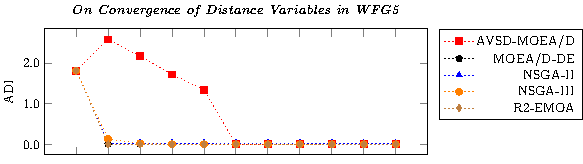
\includegraphics[scale=0.75]{images/Diversity_Long_Term_tikz_WFG5-figure0.eps}\\[0cm]%[-0.14cm] 
\hspace*{-0.08cm}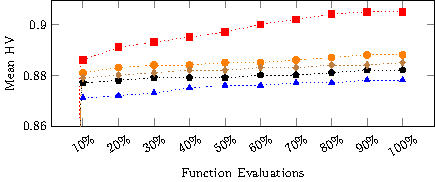
\includegraphics[scale=0.75]{images/Diversity_Long_Term_tikz_WFG5-figure1.eps}\\[0cm]%[-0.14cm] 
\end{tabular}
\caption{Diversity of distance variables (first row) and mean of \HV{} values (second row) vs. elapsed time in the bi-objective WFG5 test problem. The reported results are taken from $35$ runs.}\label{fig:WFG5_Diversity}
\end{figure}


\begin{figure}[t]
\centering
\begin{tabular}{l}
 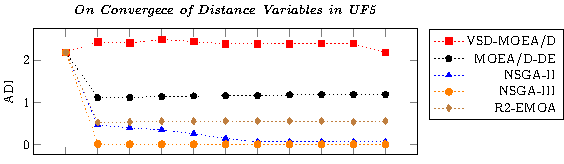
\includegraphics[scale=0.75]{images/Diversity_Long_Term_tikz_UF5-figure0.eps}\\[0cm]%[-0.14cm] 
 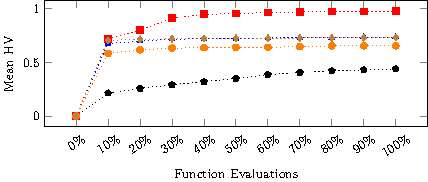
\includegraphics[scale=0.75]{images/Diversity_Long_Term_tikz_UF5-figure1.eps}\\[0cm]%[-0.14cm] 
\end{tabular}
\caption{Diversity of distance variables (first row) and mean of \HV{} values (second row) vs. elapsed time in the bi-objective UF5 test problem. The reported results are taken from $35$ runs.}\label{fig:UF5_Diversity}
\end{figure}

In order to better understand the reasons behind the benefits of \AVSDMOEAD{} against the state-of-the-art \MOEAS{},
inspecting the evolution of the \HV{} values and the diversity is quite helpful.
%
Note that in the \WFG{} test problems, the variables can be classified into two kinds of variables: 
the distance variables and the position variables.
%
A variable $x_i$ is a distance variable when for all $x$, modifying $x_i$ results in a new solution 
that dominates $x$, is equivalent to $x$, or is dominated by $x$.
%
Differently, if $x_i$ is a position variable, modifying $x_i$ in $x$ always results in a vector that is 
incomparable or equivalent to $x$~\cite{huband2006review}.
%
In order to show the behavior of the different schemes we selected WFG5 and UF5.
%
WFG5 is unimodal but its optimal region has some features that provoke stagnation in some \MOEAS{}~\cite{castillo2017multi}.
%
In contrast, the UF5 is a quite complex problem whose optimal regions are isolated in the decision variable 
space.
%
In fact its Pareto optimal front is discrete and consists of only $21$ points.
%
For each algorithm, the diversity is calculated as the average Euclidean distance among individuals (\ADI{}) in the population 
by considering only the distance variables.
%
The reason to consider only the distance variables is that in some cases premature convergence on these kinds of 
variables appear~\cite{castillo2017multi}.
%
Figures~\ref{fig:WFG5_Diversity} and~\ref{fig:UF5_Diversity} show the evolution of the ADI (top) and the mean of \HV{} (bottom) 
for the WFG5 and UF5, respectively.
%
In the WFG5 problem, the distance variables of the state-of-the-art \MOEAS{} converged to a small region 
approximately after the $10\%$ of the total execution.
%
Thus, the differential evolution operator loses it exploration power and as a result,
those \MOEAS{} were not able to improve the quality of its approximations in the remaining function evaluations. 
%
Differently, in the case of \AVSDMOEAD{} the decrease in \ADI{} is quite linear until the midpoint of the execution and
the increase of \HV{} is gradual.
%
The final \HV{} attained by \AVSDMOEAD{} is the largest one which shows the important benefit
of the gradual decrease of diversity.

As expected, promoting diversity in an explicit way is also beneficial for problems with disconnected optimal regions.
%
Attending to the data shown in Figure~\ref{fig:UF5_Diversity}, the advantage of promoting diversity in the UF5 test 
problem is clear.
%
In this case, most state-of-the-art algorithms maintain some degree of diversity in the distance variables for
the whole search.
%
However, a large degree of diversity is required to reach the 21 optimal solutions and these \MOEAS{} do not maintain
the required amount of diversity, meaning that many of the solutions are not attained.
%
In the case of \AVSDMOEAD{} the enforcement of a large degree of diversity at initial phases, promotes a larger exploration 
that enables finding additional optimal regions.
%
Once this regions are located, they are not discarded meaning that a larger level of diversity is maintained for the whole
execution.
%
This way, \AVSDMOEAD{} not only attained better \HV{} values at the first $10\%$ of total function evaluations, but 
it also kept looking for promising regions.
%
In fact, its \HV{} values improved significantly until the midpoint of the execution period i.e., the final moment
in which the diversity was explicitly promoted.
%
Then, some additional increase was attained due to the intensification in the located regions.
%
This analysis shows that the dynamics of the population depends on the problem at hand.
%
The behavior of \AVSDMOEAD{} for problems where there is a distinction between distance and position variables 
were similar to those already presented.
%
Cases where the optimal regions consists of constant values for the distance variables behaves as WFG5, whereas
the behavior for the cases where the optimal regions consist of non-constant values for the distance variables are
more similar to the UF5 case.
%
Note however, that in these cases, different levels of diversity are required, so the behavior is not so homogeneous.

\begin{figure}[t]
\centering
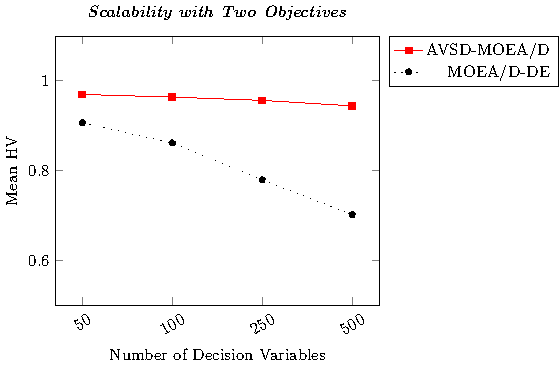
\includegraphics[scale=0.75]{images/Graphic-Scalability-2obj_tikz-figure0.eps}
\caption{Mean of the \HV{} ratio for 35 runs for the two-objective problems considering different numbers of variables}\label{fig:scalability-2obj}
\end{figure}

\begin{figure}[t]
\centering
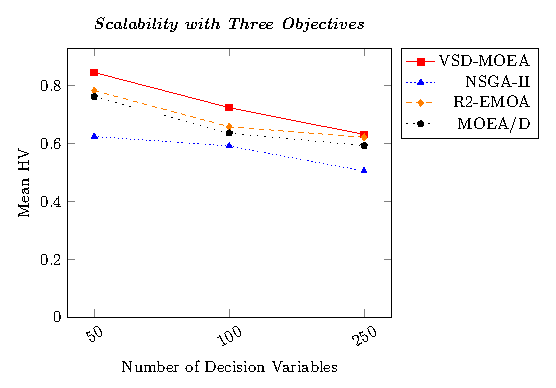
\includegraphics[scale=0.75]{images/Graphic-Scalability-3obj_tikz-figure0.eps}
\caption{Mean of the \HV{} ratio for 35 runs for the three-objective problems considering different numbers of variables} \label{fig:scalability-3obj}
\end{figure}

\subsection{Analysis of Scalability in the Decision Variables}

In order to have a better insight of the benefits of our proposal, an analysis of the scalability in terms of the number 
of decision variables is presented.
%
Given the computational cost associated to this experimentation, it was carried out considering only 
the decomposition-based algorithms.
%
\AVSDMOEAD{} and \MOEADDE{} were applied to the same benchmark problems than in the previous experiment, 
but considering $50$, $100$, $250$ and $500$ variables.
%
Note that in the WFG test problems, the number of position variables and distance variables must be specified.
%
Specifically, the number of distance variables was set to $42$, $84$, $210$ and $418$ when using $50$, $100$, $250$ and $500$ 
variables, respectively.
%
The rest of the decision variables were position variables, meaning that they were $8$, $16$, $40$ and $82$, respectively.
%
Thus, the relation between the number of position and distance variables is kept fixed.
%
In addition, the stopping criterion was set to $2.5 \times 10^7$ function evaluations.
%
Figures~\ref{fig:scalability-2obj} and~\ref{fig:scalability-3obj} show the mean \HV{} ratio for the selected algorithms, 
considering the problems with two and three objectives, respectively.
%
As expected, the \HV{} ratio decreases as the number of variables increases.
%
However, the performance of \AVSDMOEAD{} is quite robust and its decrease is less pronounced than the one in \MOEADDE{},
meaning that \AVSDMOEAD{} is specially helpful when dealing with most complex problems.
%
In fact, in our previous analyses the most remarkable performance of \AVSDMOEAD{} also appeared in the most complex cases such
as WFG8 and UF5.
%



\begin{figure}[t]
\centering
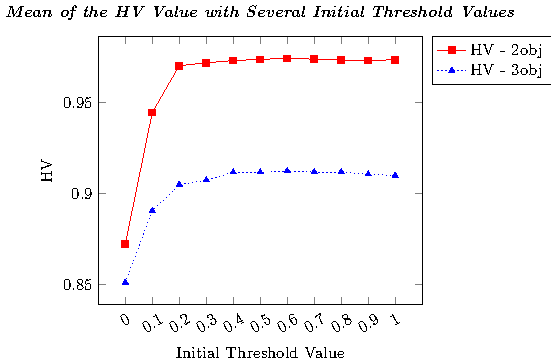
\includegraphics[scale=0.75]{images/Graphic-Initial-Distance_tikz-figure0.eps} \\
\caption{Mean of \HV{} values taking into account all the problems with several initial threshold values}\label{fig:Initial-distance-factor}
\end{figure}


\subsection{Analysis of the Initial Threshold Value}

Possibly, one of the main downsides of including a strategy to explicitly promoting the diversity 
is that this is usually at the cost of incorporating additional parameters.
%
In the case of \AVSDMOEAD{} it requires the setting of the initial threshold value ($D_I)$.
%
Given that in single-objective cases, values close to $0.4$ has attained proper performance~\cite{romero2018memetic,castillo2019differential},
$D_I = 0.4$ was used in our previous experiment.
%
This section provides a more detailed study on the implications of this parameter.
%

\begin{figure}[t]
\centering
\begin{tabular}{l}
 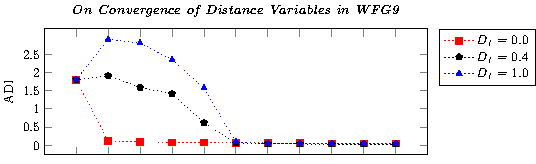
\includegraphics[scale=0.75]{images/Diversity_Long_Term_tikz_WFG9-figure0.eps}\\[0cm]%[-0.14cm] 
 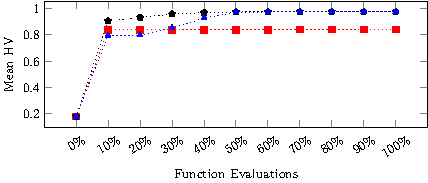
\includegraphics[scale=0.75]{images/Diversity_Long_Term_tikz_WFG9-figure1.eps}\\[0cm]%[-0.14cm] 
\end{tabular}
\caption{Diversity of distance variables (first row) and mean of \HV{} values (second row) vs. elapsed time in the two-objective WFG9 test problem. The reported results are taken from $35$ runs.}\label{fig:WFG9_Diversity}
\end{figure}


%\begin{figure}[t]
%\centering
%\begin{tabular}{l}
% 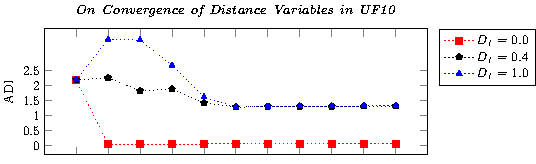
\includegraphics[scale=0.75]{images/Diversity_Long_Term_tikz_UF10-figure0.eps}\\[0cm]%[-0.14cm] 
% 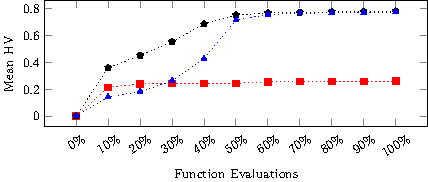
\includegraphics[scale=0.75]{images/Diversity_Long_Term_tikz_UF10-figure1.eps}\\[0cm]%[-0.14cm] 
%\end{tabular}
%\caption{Diversity of distance variables (first row) and mean of \HV{} values (second row) vs. elapsed time in the three-objective UF10 test problem. The reported results are taken from $35$ runs.}\label{fig:UF10_Diversity}
%\end{figure}

In order to better understand the importance of $D_I$, the whole set of benchmark problems was tested with different values
of $D_I$.
%
As in previous experiments, the stopping criterion was set to $2.5 \times 10^7$ function evaluations.
%
Since normalized distances are used (see~\ref{eqn:distance}), the maximum attainable distance is $1.0$, while
the minimum one is $0$, which implies not promoting diversity in the variable space.
%
Thus, several values in this range were considered.
%
Specifically, the values $D_I = \{0.0, 0.1, 0.2, 0.3, 0.4, 0.5, 0.6, 0.7, 0.8, 0.9, 1.0\}$ were tested.

Figure~\ref{fig:Initial-distance-factor} shows the mean \HV{} ratio obtained for both the two-objective 
and the three-objective case with the tested $D_I$ values.
%
The worst performance of the \AVSDMOEAD{} is when it is set to $D_I=0.0$.
%
The \HV{} ratio obtained quickly increases as higher $D_I$ values up to $0.2$ are used.
%
Larger values provide a quite similar performance.
%
Thus, there is a wide range of values (from $0.2$ to $1.0$) where a really good performance is attained, 
meaning that the behavior of \AVSDMOEAD{} is quite robust.
%
Thus, properly setting this parameter is not a complex task.

In order to better understand the implications of $D_I$ on the dynamics of the population Figure~\ref{fig:WFG9_Diversity}
shows for \AVSDMOEAD{} the evolution of diversity on the distance variables for three different values of $D_I$.
%
When using $D_I = 0$, the diversity is reduced quite fastly which results in premature convergence.
%
Thus, a not too high hypervolume is attained.
%
However, when using $D_I = 0.4$ and $D_I = 1$ the loss of diversity is slowed down and practically a perfect hypervolume
is attained.
%
Note that the setting of $D_I = 1$ promotes a larger diversity so the hypervolume increases slower than when using
$D_I = 0.4$.
%
However, the exploration degree in both cases is enough to reach high-quality solutions.
%
The behavior is quite similar in all problems, which explains the stability of the algorithms for
different $D_I$ values.
%
Note that probably, for shorter periods the setting of a proper $D_I$ value might be much more important.
%
However, at least for long-term executions, practically any value larger than $0.2$ attains similar solutions,
which we consider a quite positive feature.


%Thereafter, in a more specifically way, the effect of this parameter is analized in WFG9 and UF10 test problems, in two and three objectives, respectively.
%
%In the same way than in the previous experiments, the Figures and~\ref{fig:UF10_Diversity} show the evolution of diversity (top side) and \HV{} ratio (bottom side) among the execution.
%
%The WFG9 test problem is multi-modal and deceptive.
%
%In addition, the UF10 test problem is highly multi-frontal and can be considered as one of the most challenging problems.
%
%Such diagrams belong to \AVSDMOEAD{} with the values $D_I = \{0.0, 0.4, 1.0\}$.
%
%Interestingly, the behavior of \AVSDMOEAD{} with $D_I=0.0$ is quite similar than the state-of-the-art \MOEAS{}, which confirms or previous claim.
%
%The motivation behind those diagrams is to ilustrate that to achieve a better balance between exploration and exploitation can be the explicit promotion of diversity among the execution.
%
%Therefore, those figures show that in multi-objective optimization --depending in each \MOP{}-- there is a relation between the diversity and the quality solutions, in fact visually the shapes of the \ADI{} and \HV{} ratio complement each other.
%
%Even more the \HV{} ratio values are constantly improving as the execution time elapses.
%


